%!TEX root = ../thesis_phd.tex
%%%%%%%%%%%%%%%%%%%%%%%%%%%%%%%%%%%%%%%%%%%%%%%%%%%%%%%%%%%%%%%%%%%%%%%%%%%%%%%%
%%%%%%%%%%%%%%%%%%%%%%%%%%%%%%%%%%%%%%%%%%%%%%%%%%%%%%%%%%%%%%%%%%%%%%%%%%%%%%%%
% conclusion.tex:
%%%%%%%%%%%%%%%%%%%%%%%%%%%%%%%%%%%%%%%%%%%%%%%%%%%%%%%%%%%%%%%%%%%%%%%%%%%%%%%%
\chapter{Results}
\label{results_chapter}
%%%%%%%%%%%%%%%%%%%%%%%%%%%%%%%%%%%%%%%%%%%%%%%%%%%%%%%%%%%%%%%%%%%%%%%%%%%%%%%%


Upon opening the signal region for analysis, 39 events were selected.
Assuming the default oscillation parameters,
shown in Table \ref{osc_par_table}, the extrapolated prediction
was for 38.1 \numi beam events to be selected with a cosmic ray background
of 3.4 events.
In the absence of neutrino oscillation, 222.0 \numi beam events would have been
predicted.
The selected spectrum was fit as described
in Section \ref{fitting_section}; the best-fit parameters are
$\sin^2(\thetatth) = 0.43$ (with a statistically-degenerate compliment at 0.60)
and
$|\deltamtht| = 2.48\times10^{-3}~\text{eV}^2$.
The fit results will be discussed in more detail in Section
\ref{fit_results_section}.


\begin{figure}
\begin{center}
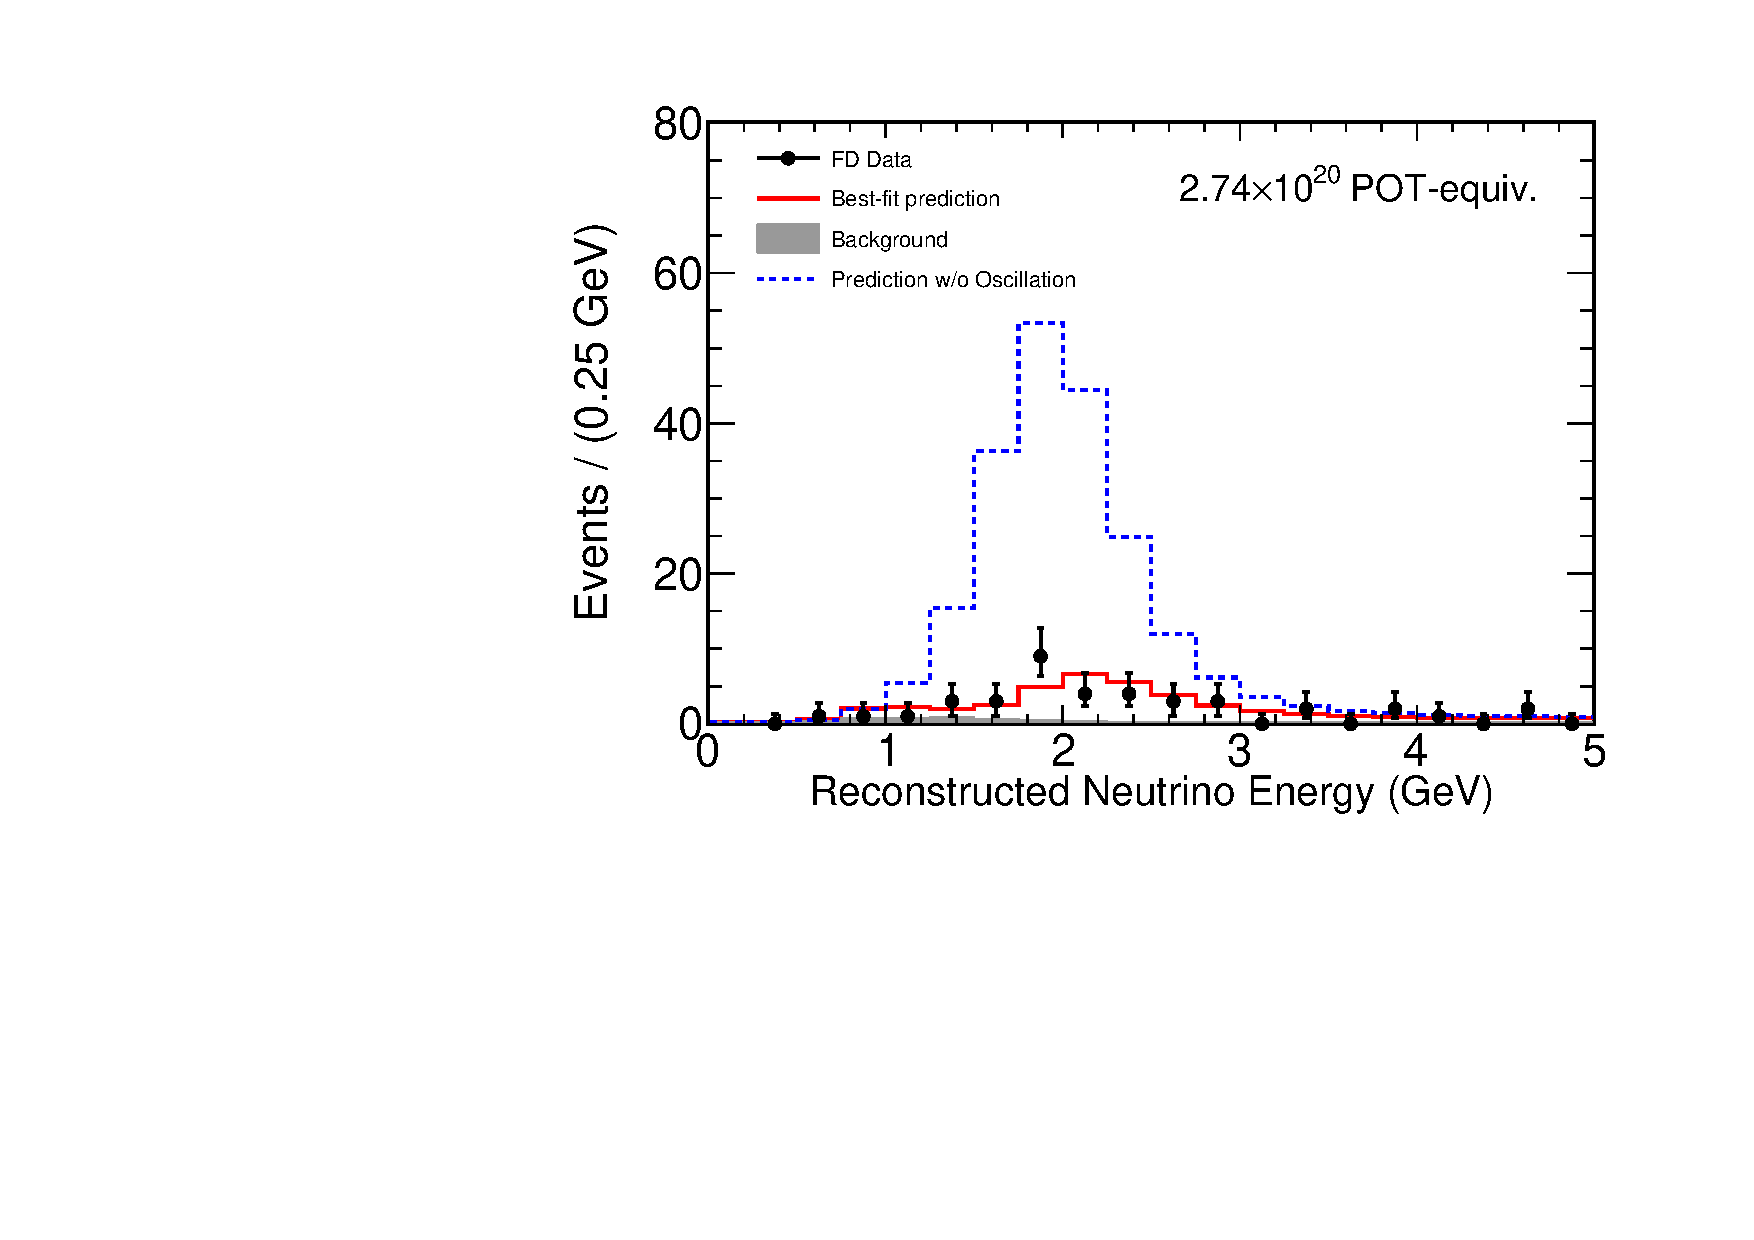
\includegraphics[width=\textwidth]{figures/results/fd_data_mc_numi_plots/ccE_unblind_wUnosc.pdf}
\end{center}
\caption{FD observed spectrum with prediction in the absence of neutrino oscillation}{
The distribution of the 39 selected FD events are shown shown in black.
The selected spectrum was fit to obtain the oscillation parameters used
for the FD MC prediction shown in red, while
the blue dashed line shows the FD MC prediction in the absence neutrino
oscillation.
The background spectrum is shown in gray.
}
\label{selected_spectrum_with_unosc}

\end{figure}


\section{FD Selected Sample}
\label{fd_selection_section}

It is important to inspect the selected events to confirm that
the selection is consistent with expectation.
For a variety of distributions which characterize the selection,
we can compare the distribution from selected FD events
to the FD MC prediction.
The following distributions can all be seen in their respective figures:
\begin{itemize}
  \item CNN softmax output (Figure \ref{cvn_unblind})
  \item Slice \nhit (Figure \ref{nhit_unblind})
  \item Number of tracks formed by KalmanTrack (Figure \ref{nkal_unblind})
  \item Muon track length (Figure \ref{trkLength_unblind})
  \item Muon track start $X$ (Figure \ref{trkStartX_unblind})
  \item Muon track start $Y$ (Figure \ref{trkStartY_unblind})
  \item Muon track start $Z$ (Figure \ref{trkStartZ_unblind})
  \item Muon track stop $X$ (Figure \ref{trkEndX_unblind})
  \item Muon track stop $Y$ (Figure \ref{trkEndY_unblind})
  \item Muon track stop $Z$ (Figure \ref{trkEndZ_unblind})
  \item Muon track $Z$-direction cosine (Figure \ref{dirZ_unblind})
  \item Hadronic cluster \nhit (Figure \ref{hadNhit_unblind})
  \item Hadronic energy (Figure \ref{hadEshift_unblind})
  \item Muon ID (Figure \ref{remid_unblind}).
\end{itemize}
None of the distributions show significant excursions relative to the
MC prediction.
The consistency between FD data and the MC prediction provides
a reasonable measure of confidence in the event selection,
although it is hard to make a very strong statement
with such limited statistics.




\begin{figure}
\begin{center}
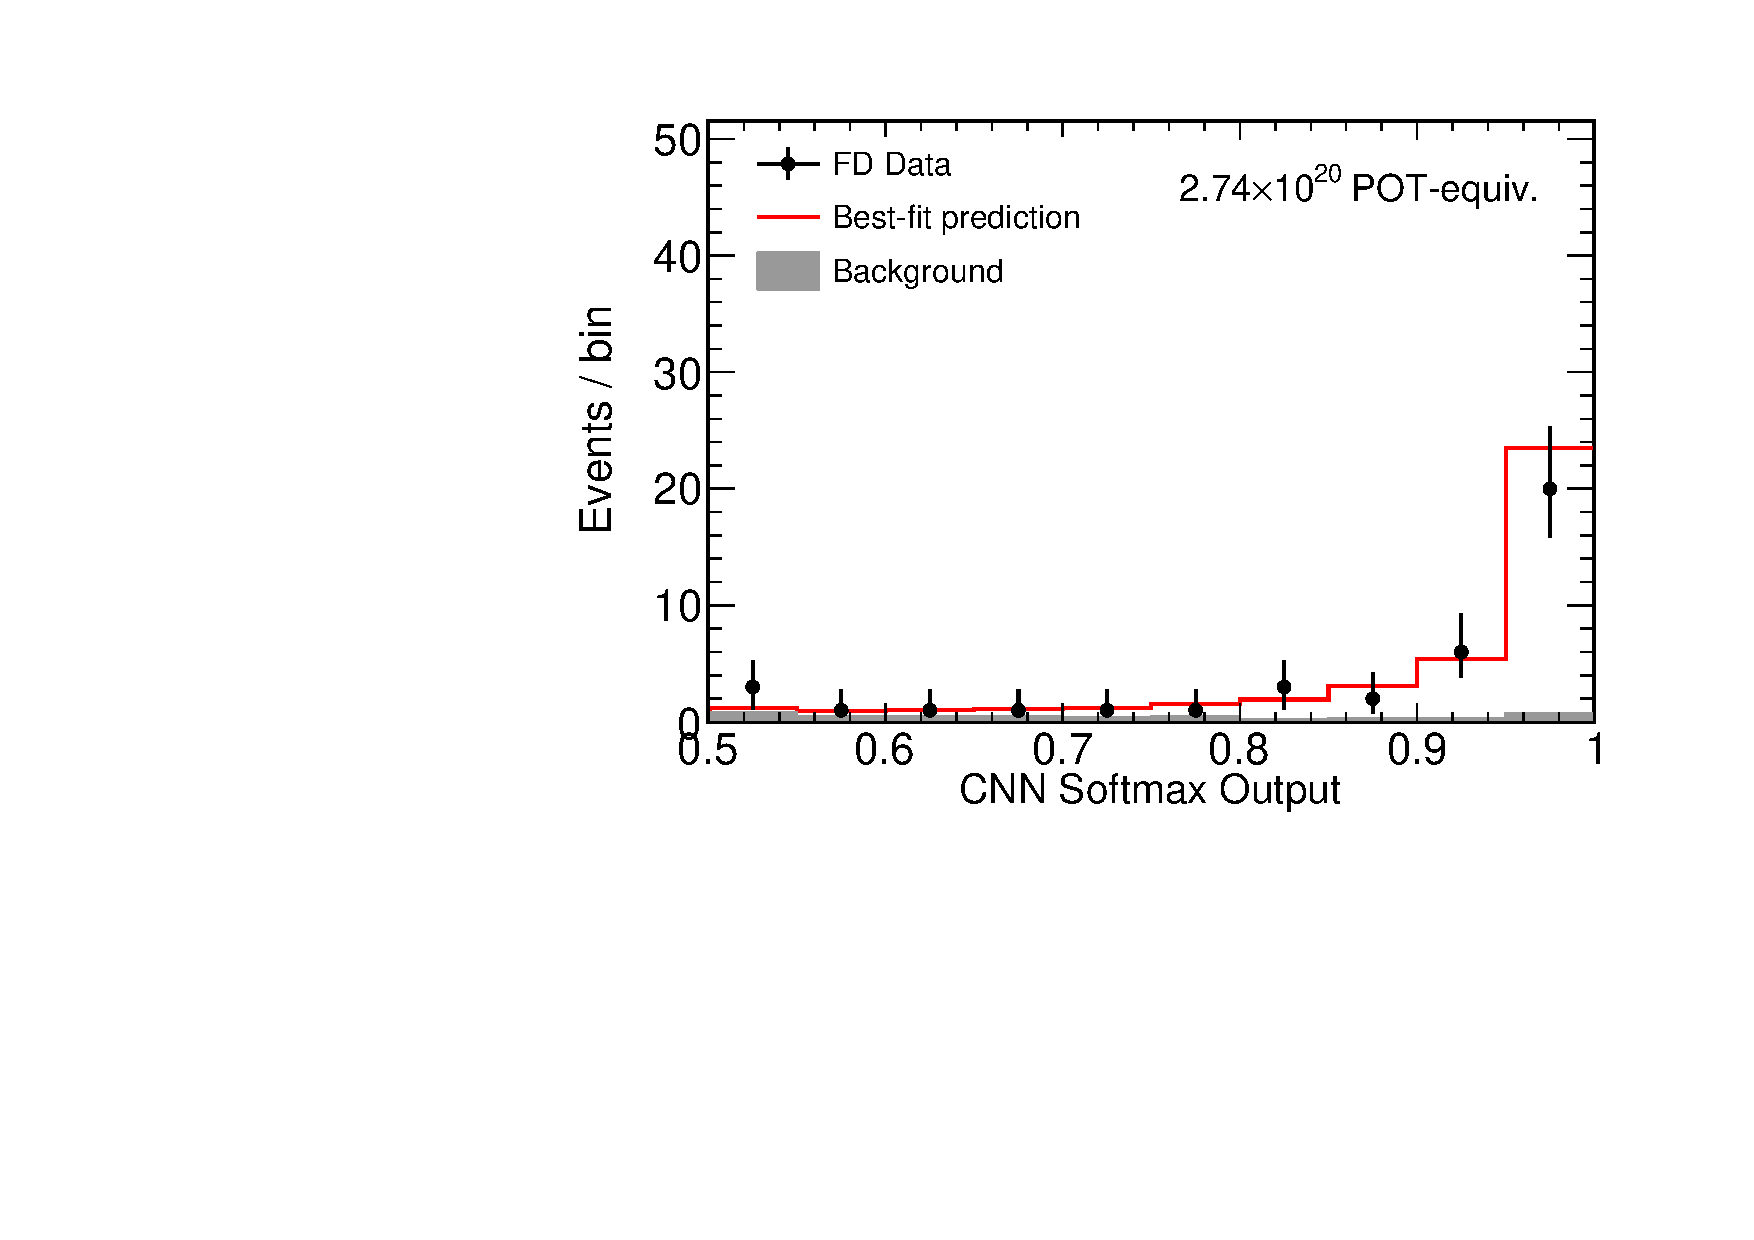
\includegraphics[width=\textwidth]{figures/results/fd_data_mc_numi_plots/cvn_unblind.pdf}
\end{center}
\caption{ CNN softmax output distribution for selected FD events with MC prediction }{
The distribution of the 39 selected FD events are shown shown in black.
The selected spectrum was fit to obtain the oscillation parameters used
for the FD MC prediction shown in red, while
the blue dashed line shows the FD MC prediction in the absence neutrino
oscillation.
The background spectrum is shown in gray.
}
\label{cvn_unblind}

\end{figure}



\begin{figure}
\begin{center}
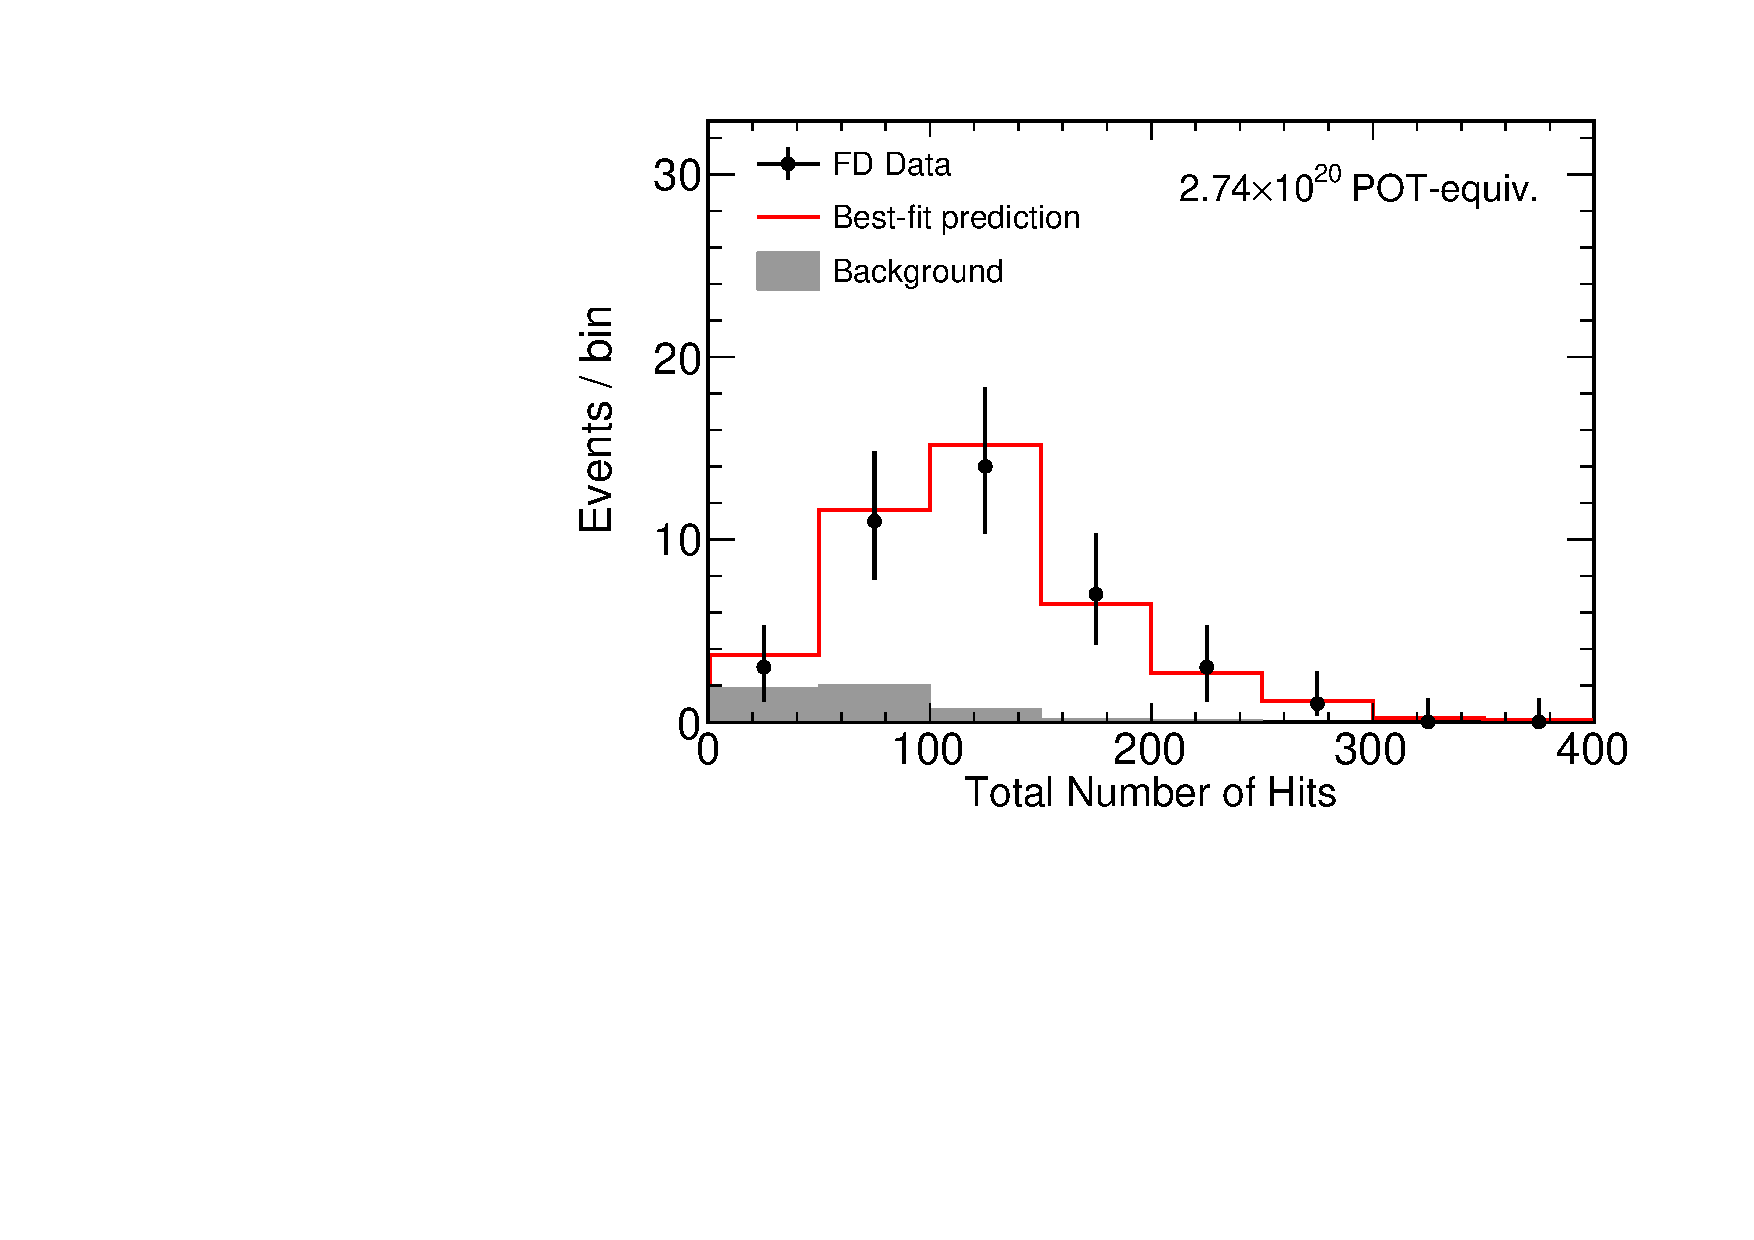
\includegraphics[width=\textwidth]{figures/results/fd_data_mc_numi_plots/nhit_unblind.pdf}
\end{center}
\caption{  Slice \nhit distribution for selected FD events with MC prediction }{
The distribution of the 39 selected FD events are shown shown in black.
The selected spectrum was fit to obtain the oscillation parameters used
for the FD MC prediction shown in red, while
the blue dashed line shows the FD MC prediction in the absence neutrino
oscillation.
The background spectrum is shown in gray.
}
\label{nhit_unblind}

\end{figure}



\begin{figure}
\begin{center}
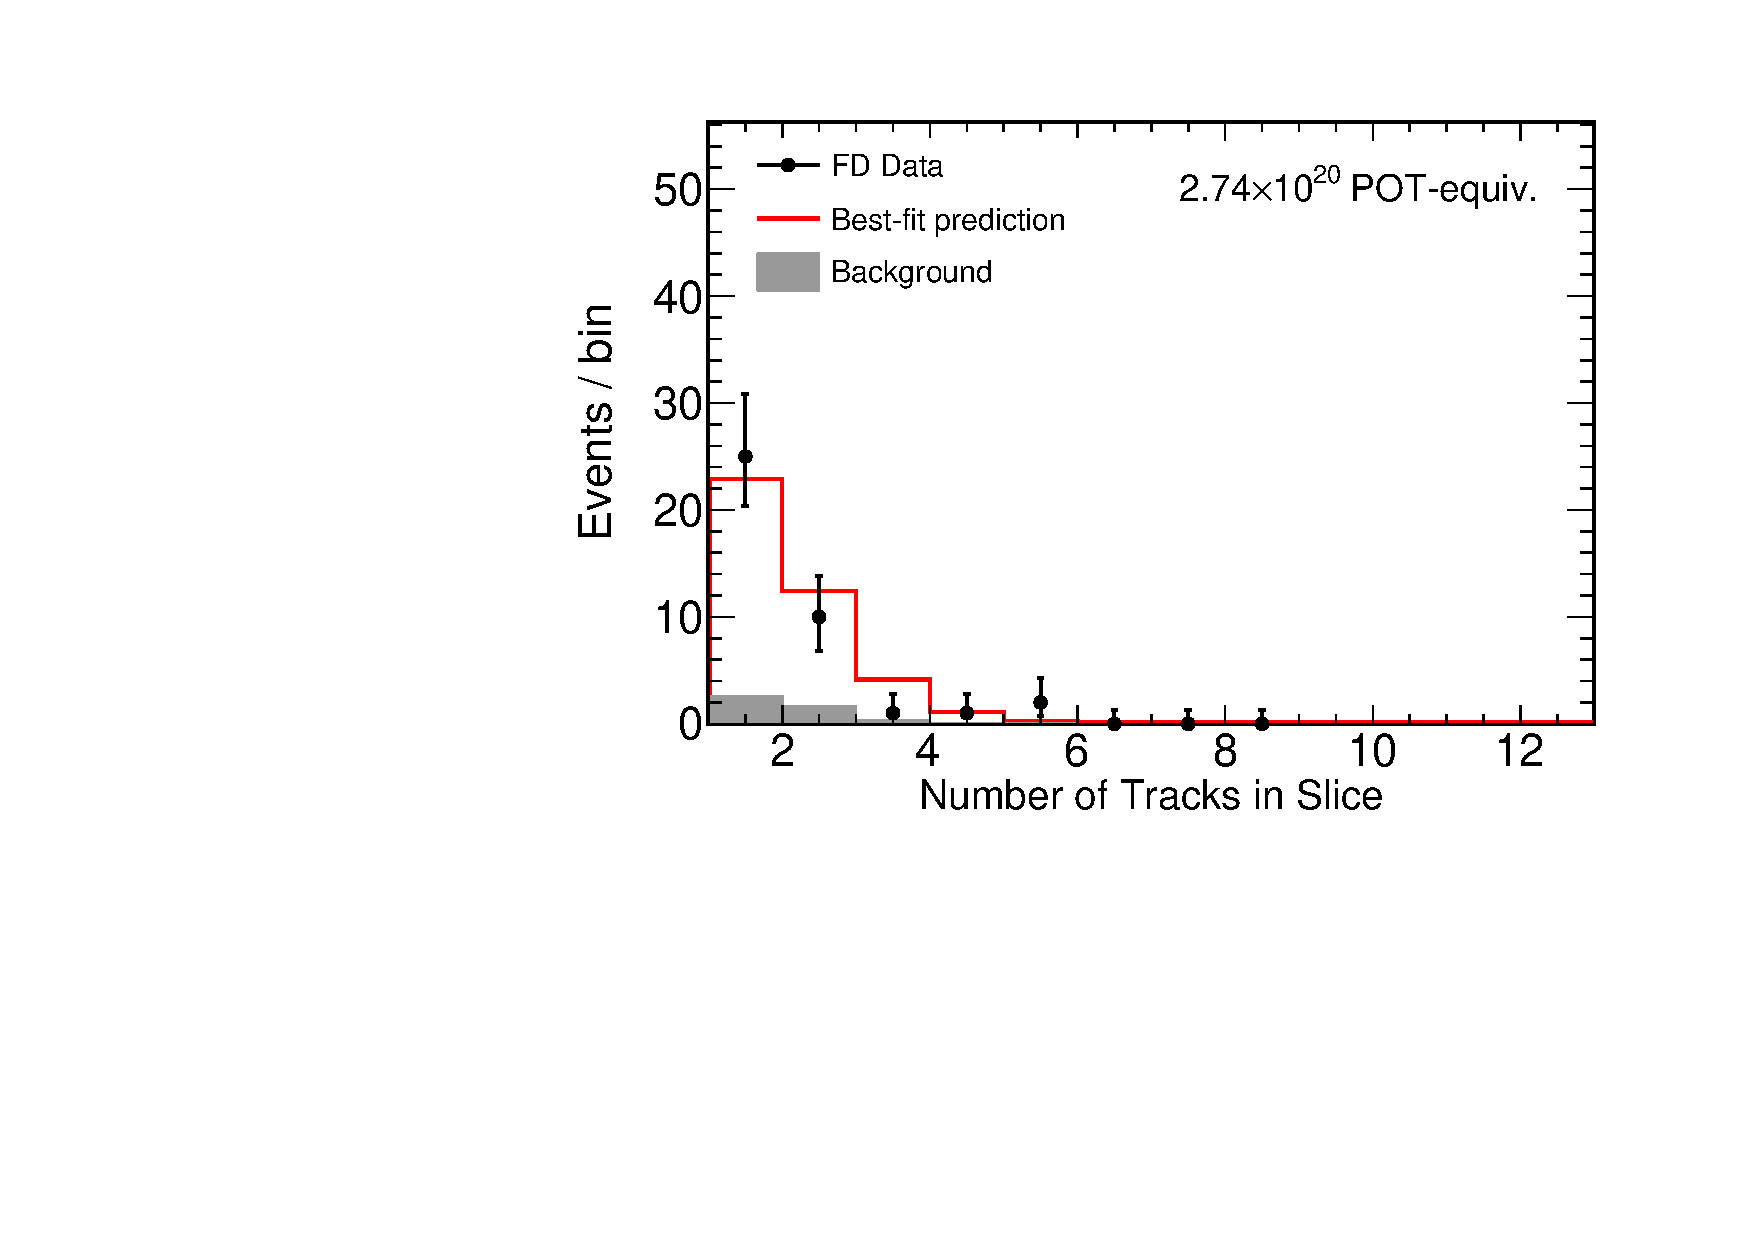
\includegraphics[width=\textwidth]{figures/results/fd_data_mc_numi_plots/nkal_unblind.pdf}
\end{center}
\caption{  Number of tracks formed by KalmanTrack distribution for selected FD events with MC prediction }{
The distribution of the 39 selected FD events are shown shown in black.
The selected spectrum was fit to obtain the oscillation parameters used
for the FD MC prediction shown in red, while
the blue dashed line shows the FD MC prediction in the absence neutrino
oscillation.
The background spectrum is shown in gray.
}
\label{nkal_unblind}

\end{figure}



\begin{figure}
\begin{center}
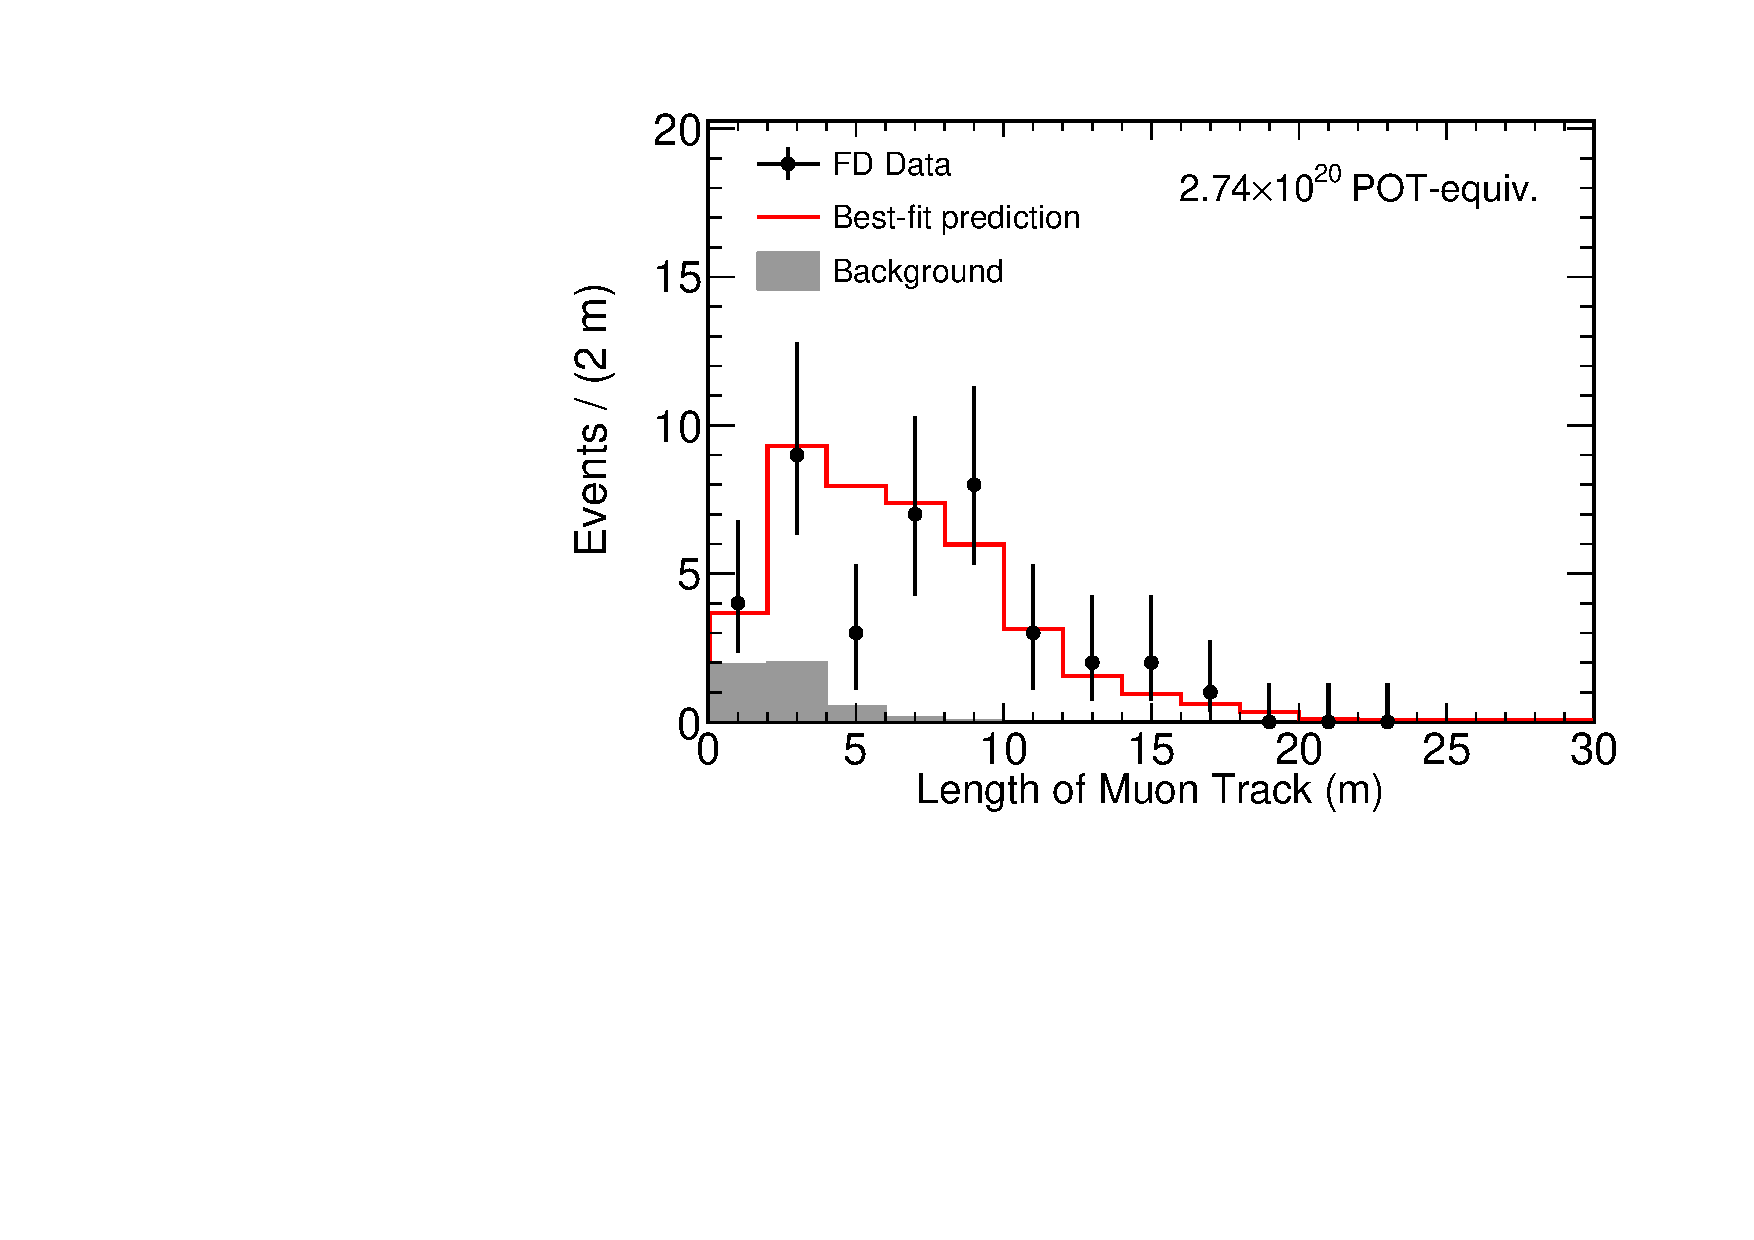
\includegraphics[width=\textwidth]{figures/results/fd_data_mc_numi_plots/trkLength_unblind.pdf}
\end{center}
\caption{Muon track length distribution for selected FD events
with MC prediction }{
The distribution of the 39 selected FD events are shown shown in black.
The selected spectrum was fit to obtain the oscillation parameters used
for the FD MC prediction shown in red, while
the blue dashed line shows the FD MC prediction in the absence neutrino
oscillation.
The background spectrum is shown in gray.
}
\label{trkLength_unblind}

\end{figure}



\begin{figure}
\begin{center}
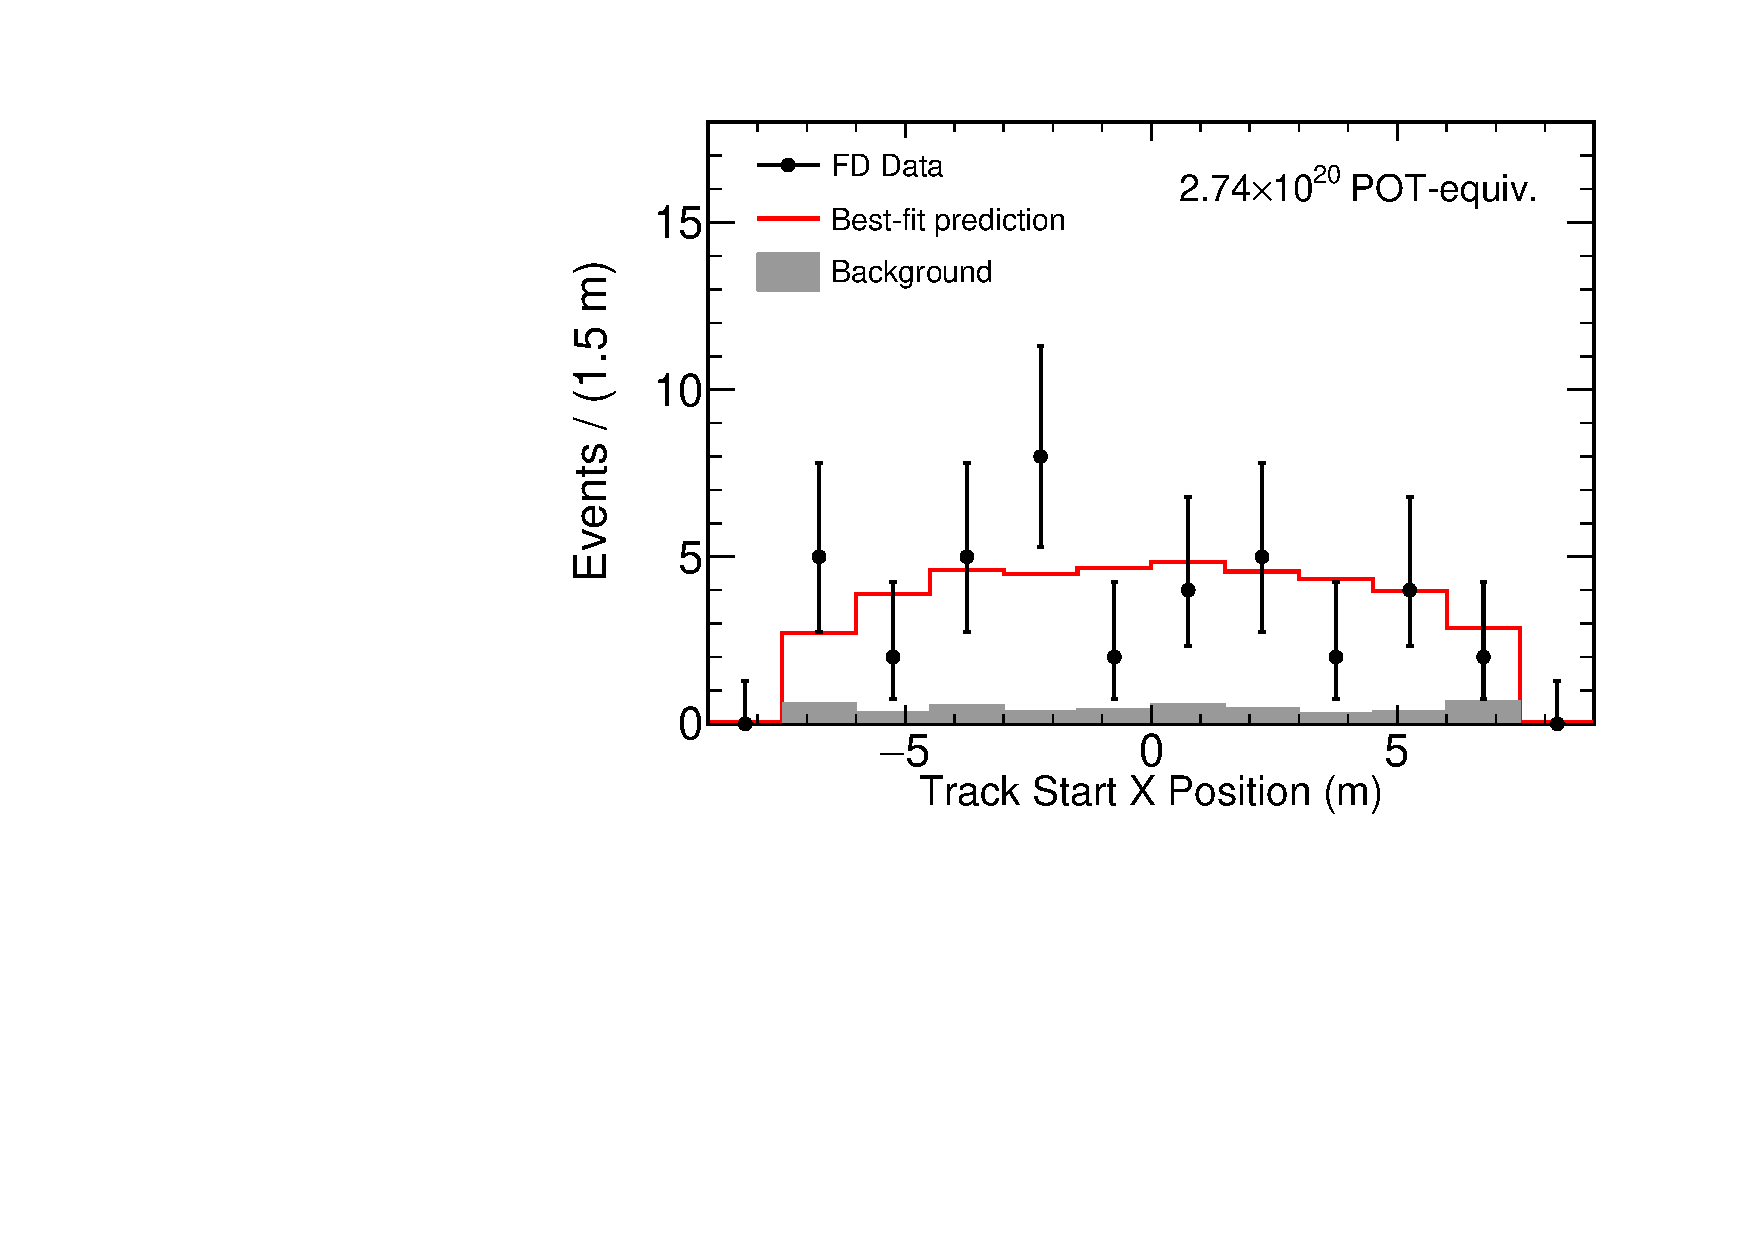
\includegraphics[width=\textwidth]{figures/results/fd_data_mc_numi_plots/trkStartX_unblind.pdf}
\end{center}
\caption{ Muon track start $X$ distribution for selected FD events with MC prediction }{
The distribution of the 39 selected FD events are shown shown in black.
The selected spectrum was fit to obtain the oscillation parameters used
for the FD MC prediction shown in red, while
the blue dashed line shows the FD MC prediction in the absence neutrino
oscillation.
The background spectrum is shown in gray.
}
\label{trkStartX_unblind}

\end{figure}



\begin{figure}
\begin{center}
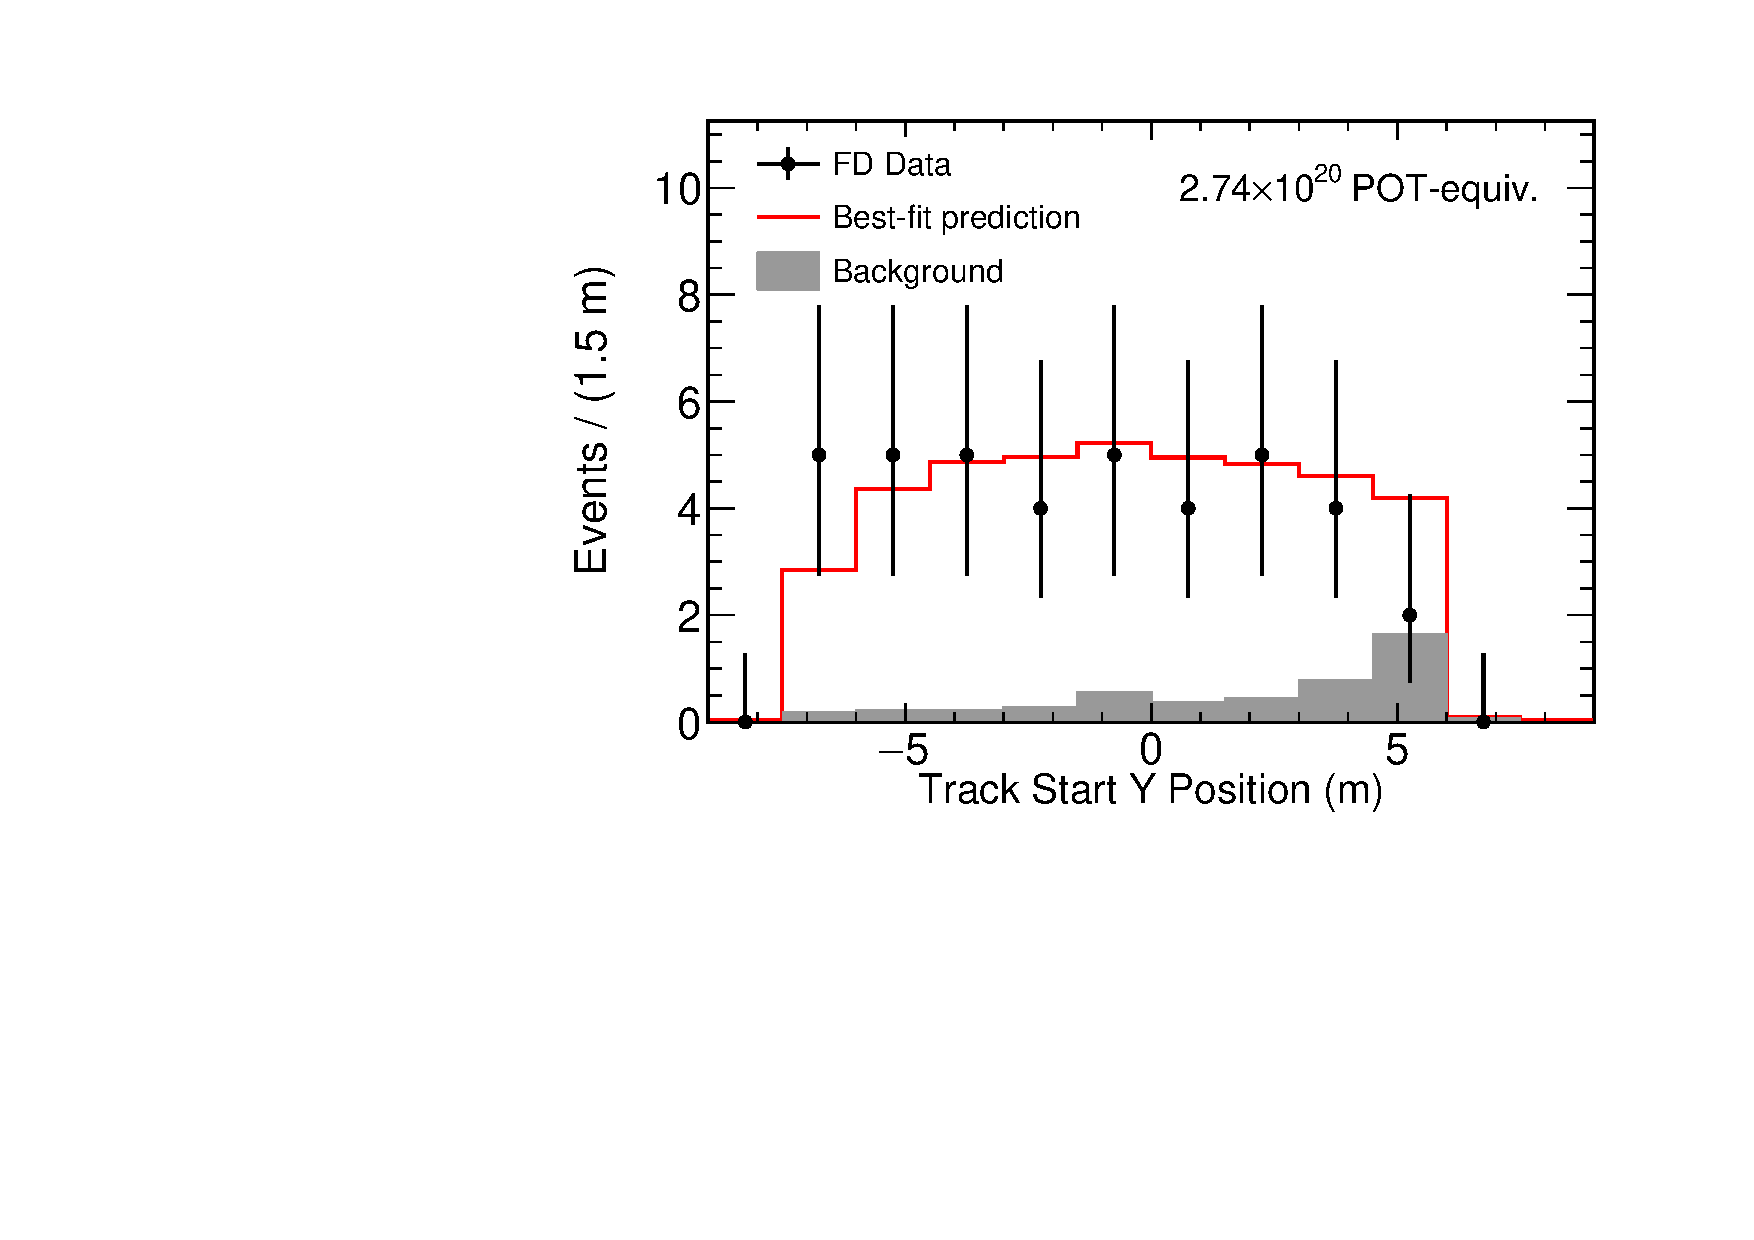
\includegraphics[width=\textwidth]{figures/results/fd_data_mc_numi_plots/trkStartY_unblind.pdf}
\end{center}
\caption{ Muon track start $Y$ distribution for selected FD events with MC prediction }{
The distribution of the 39 selected FD events are shown shown in black.
The selected spectrum was fit to obtain the oscillation parameters used
for the FD MC prediction shown in red, while
the blue dashed line shows the FD MC prediction in the absence neutrino
oscillation.
The background spectrum is shown in gray.
}
\label{trkStartY_unblind}

\end{figure}



\begin{figure}
\begin{center}
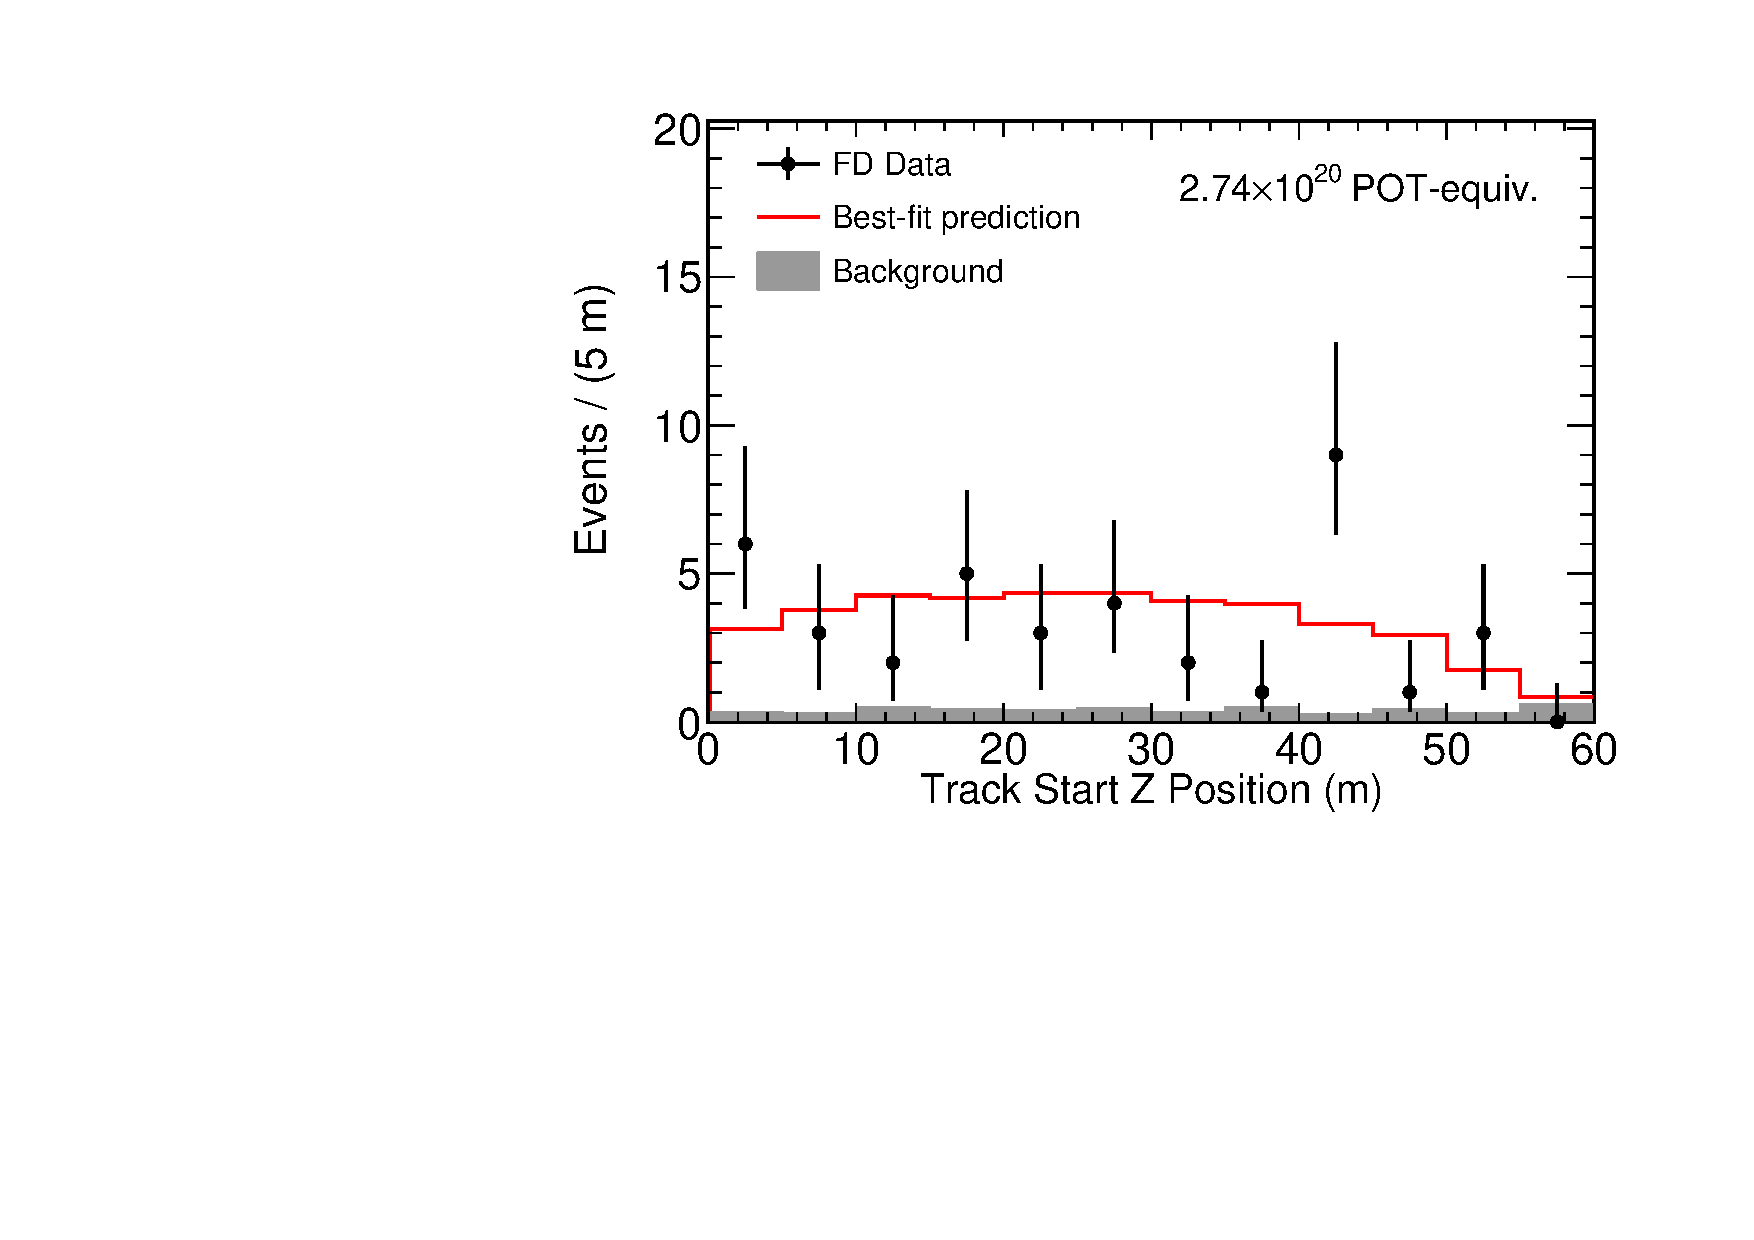
\includegraphics[width=\textwidth]{figures/results/fd_data_mc_numi_plots/trkStartZ_unblind.pdf}
\end{center}
\caption{ Muon track start $Z$ distribution for selected FD events with MC prediction }{
The distribution of the 39 selected FD events are shown shown in black.
The selected spectrum was fit to obtain the oscillation parameters used
for the FD MC prediction shown in red, while
the blue dashed line shows the FD MC prediction in the absence neutrino
oscillation.
The background spectrum is shown in gray.
}
\label{trkStartZ_unblind}

\end{figure}


\begin{figure}
\begin{center}
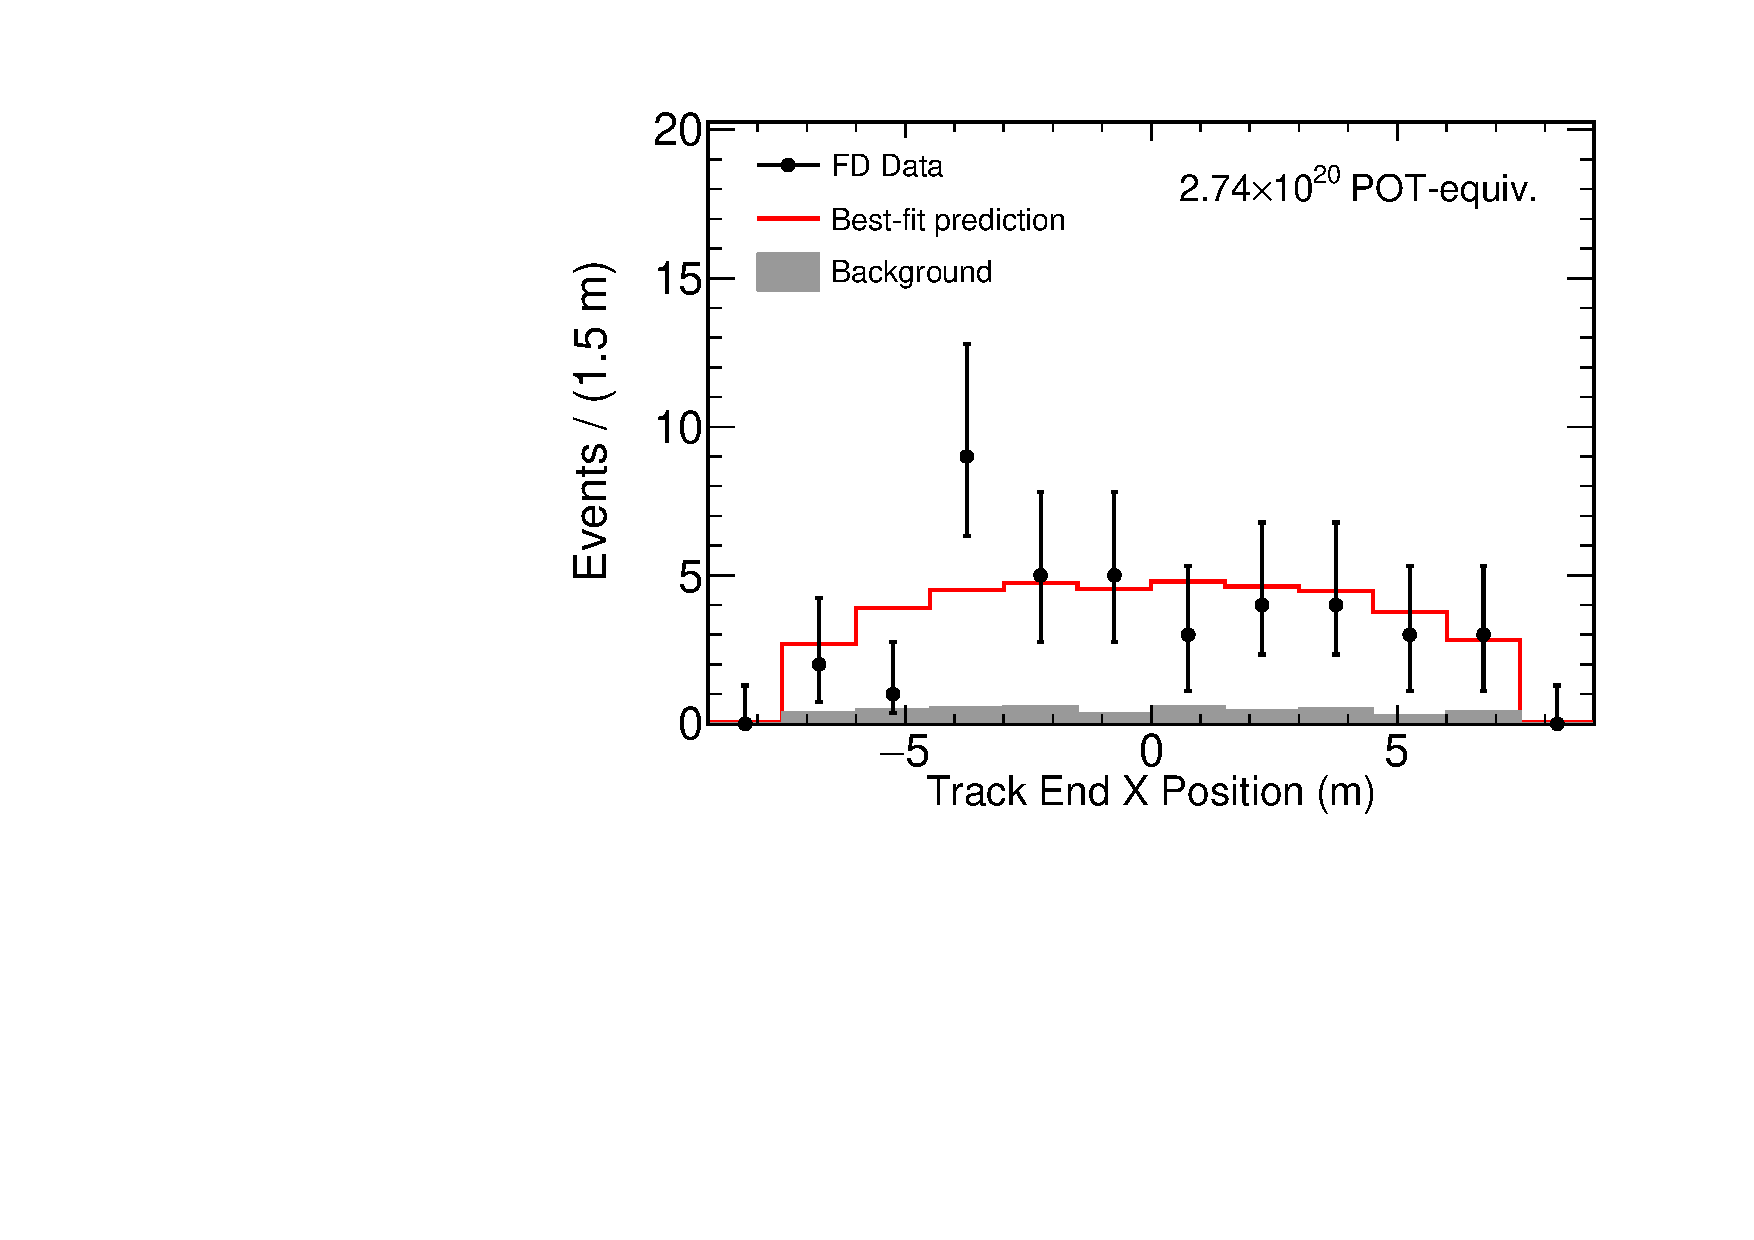
\includegraphics[width=\textwidth]{figures/results/fd_data_mc_numi_plots/trkEndX_unblind.pdf}
\end{center}
\caption{ Muon track stop $X$ distribution for selected FD events with MC prediction }{
The distribution of the 39 selected FD events are shown shown in black.
The selected spectrum was fit to obtain the oscillation parameters used
for the FD MC prediction shown in red, while
the blue dashed line shows the FD MC prediction in the absence neutrino
oscillation.
The background spectrum is shown in gray.
}
\label{trkEndX_unblind}

\end{figure}



\begin{figure}
\begin{center}
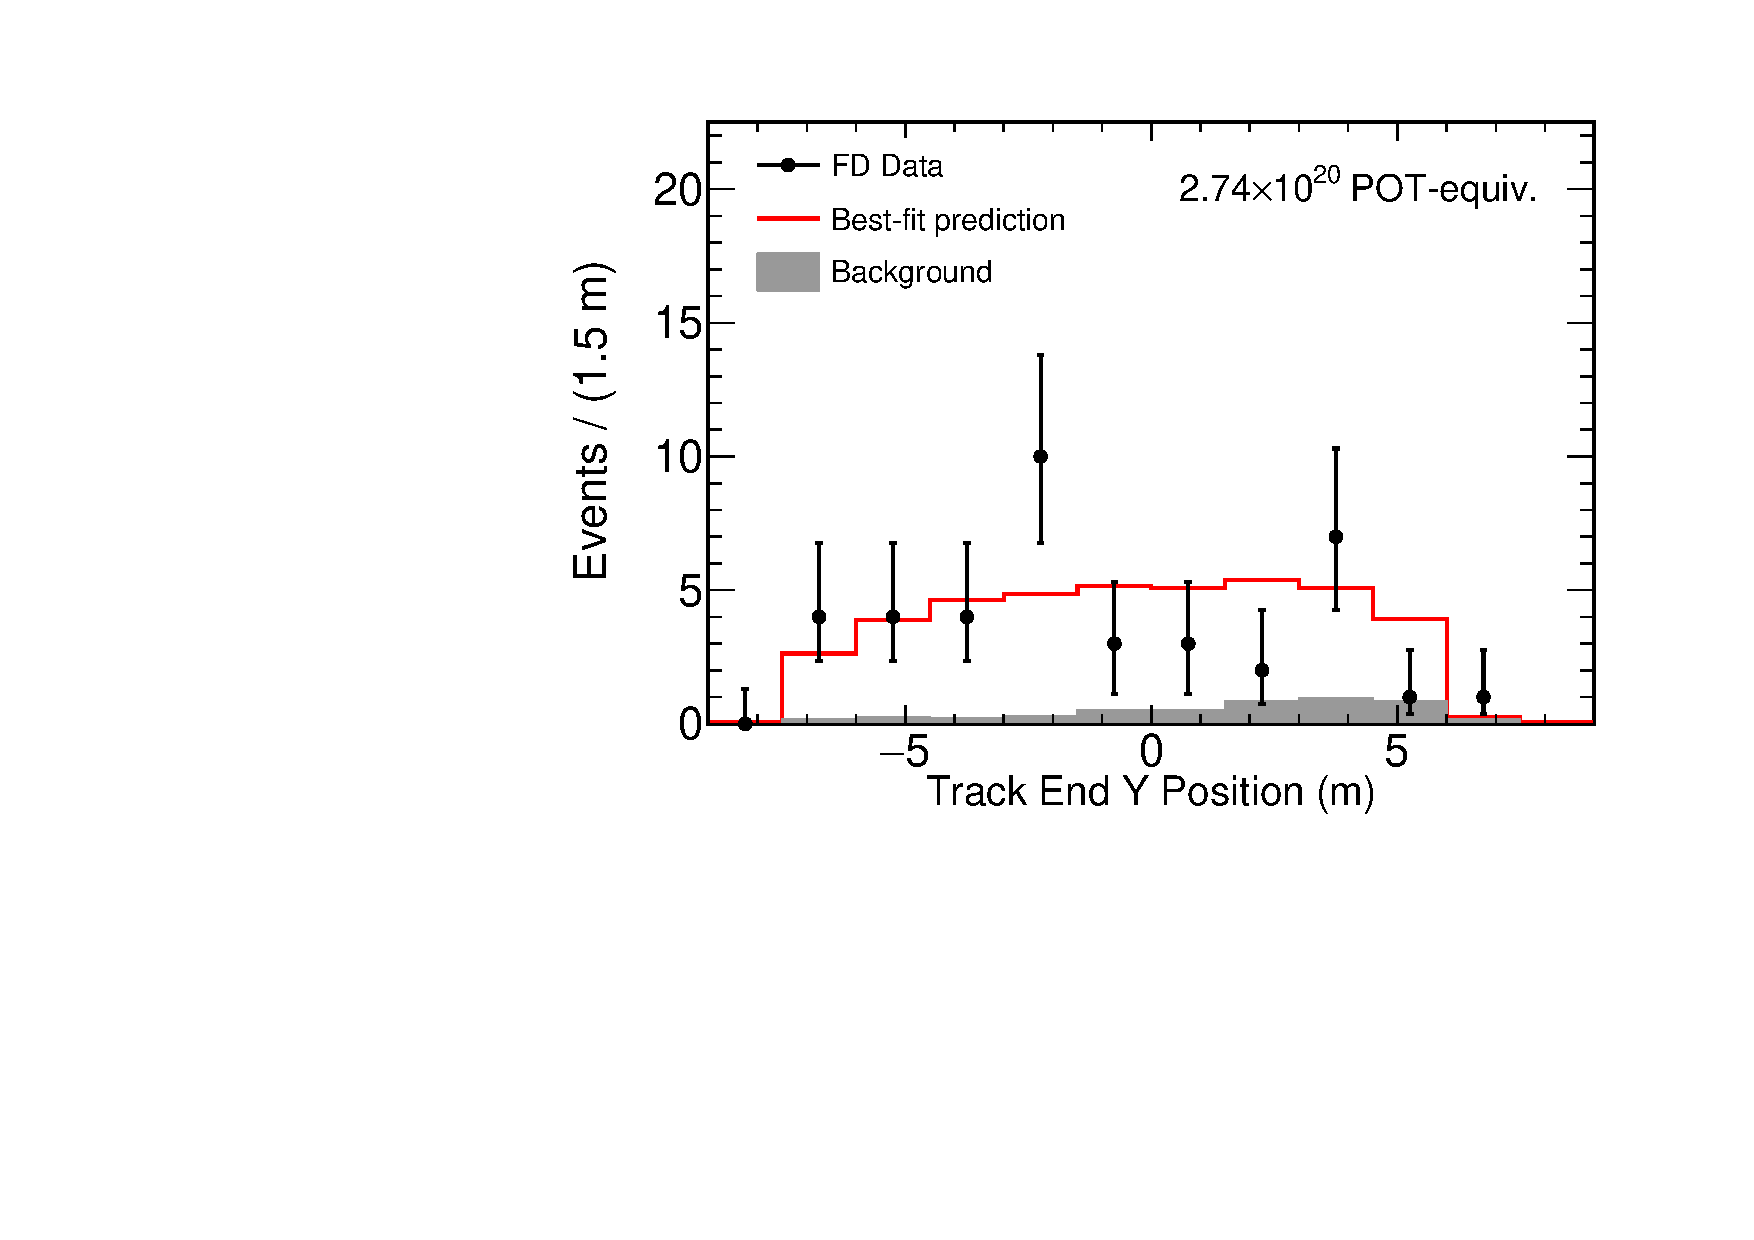
\includegraphics[width=\textwidth]{figures/results/fd_data_mc_numi_plots/trkEndY_unblind.pdf}
\end{center}
\caption{ Muon track stop $Y$ distribution for selected FD events with MC prediction }{
The distribution of the 39 selected FD events are shown shown in black.
The selected spectrum was fit to obtain the oscillation parameters used
for the FD MC prediction shown in red, while
the blue dashed line shows the FD MC prediction in the absence neutrino
oscillation.
The background spectrum is shown in gray.
}
\label{trkEndY_unblind}

\end{figure}



\begin{figure}
\begin{center}
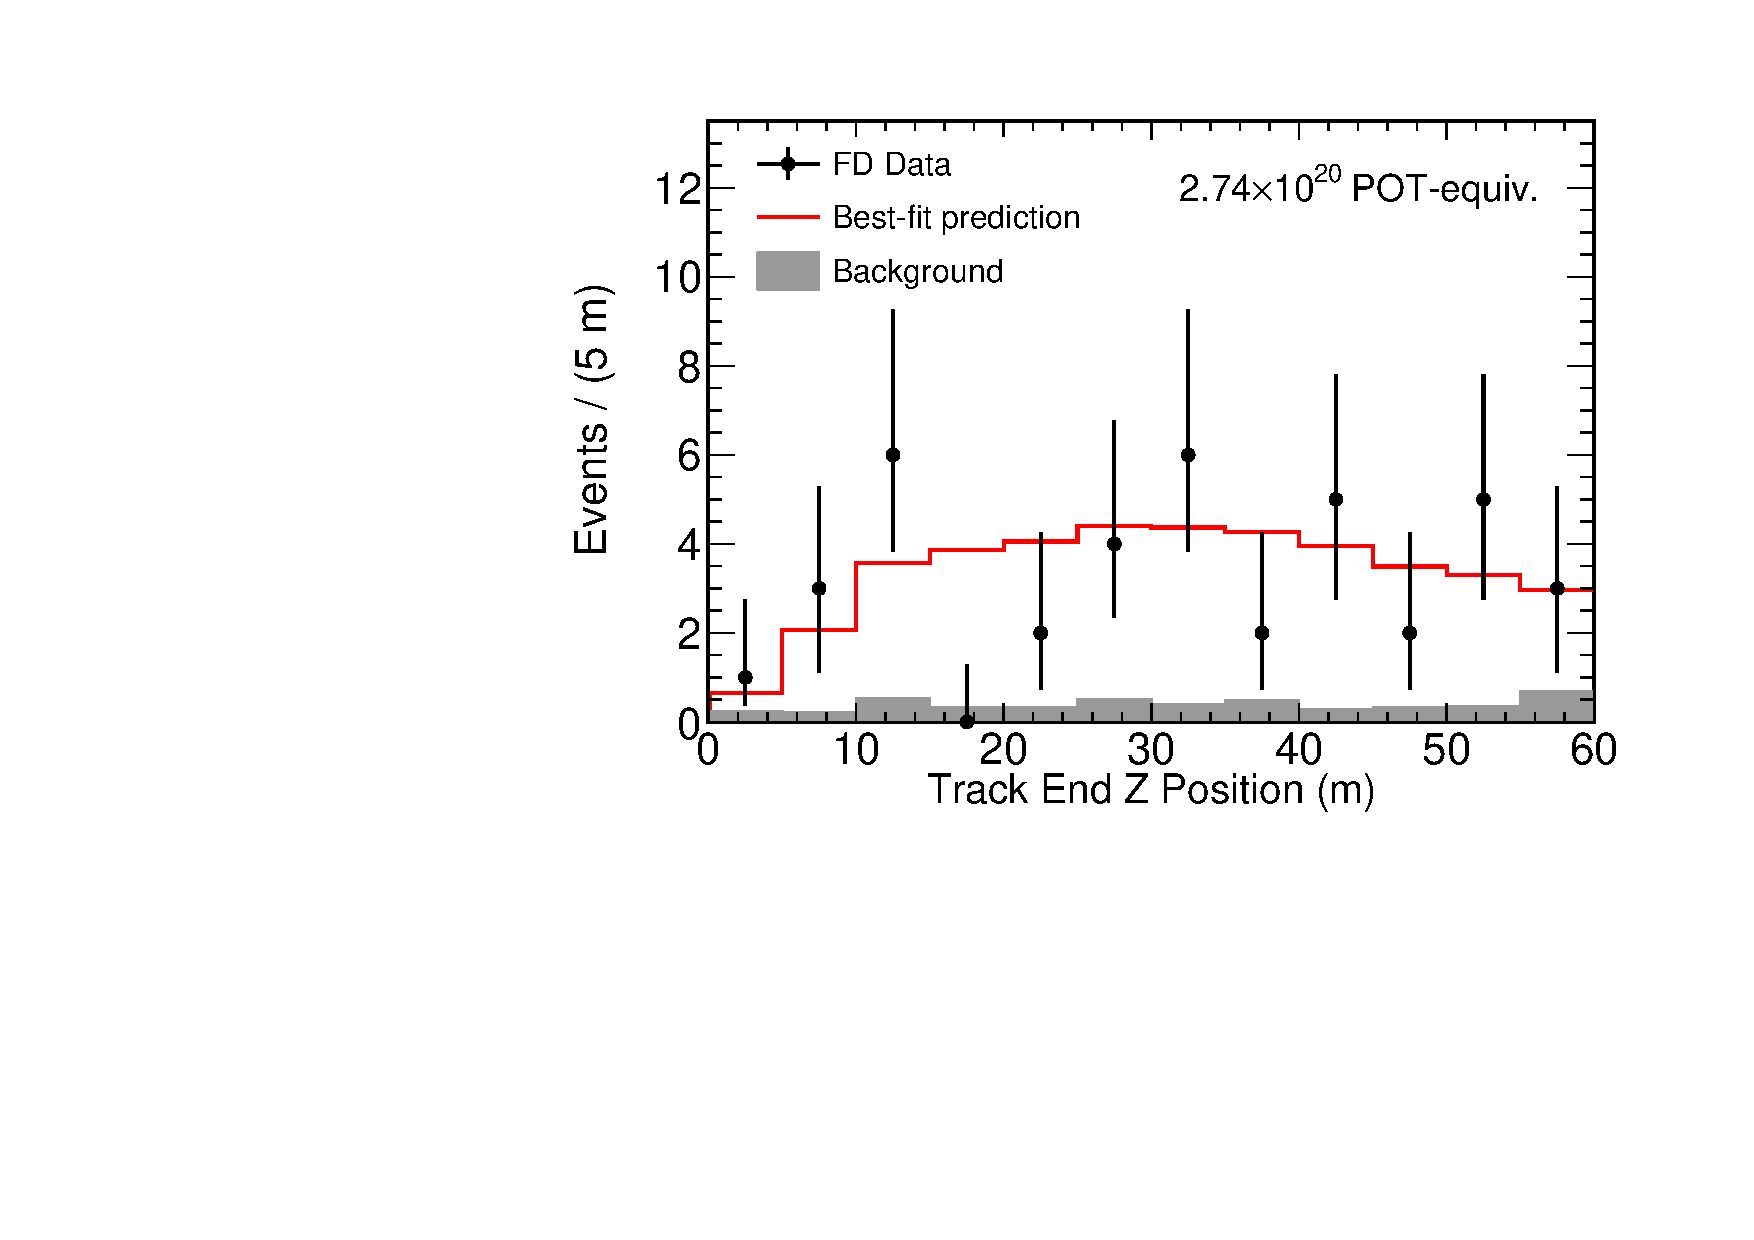
\includegraphics[width=\textwidth]{figures/results/fd_data_mc_numi_plots/trkEndZ_unblind.pdf}
\end{center}
\caption{ Muon track stop $Z$ distribution for selected FD events with MC prediction }{
The distribution of the 39 selected FD events are shown shown in black.
The selected spectrum was fit to obtain the oscillation parameters used
for the FD MC prediction shown in red, while
the blue dashed line shows the FD MC prediction in the absence neutrino
oscillation.
The background spectrum is shown in gray.
}
\label{trkEndZ_unblind}

\end{figure}




\begin{figure}
\begin{center}
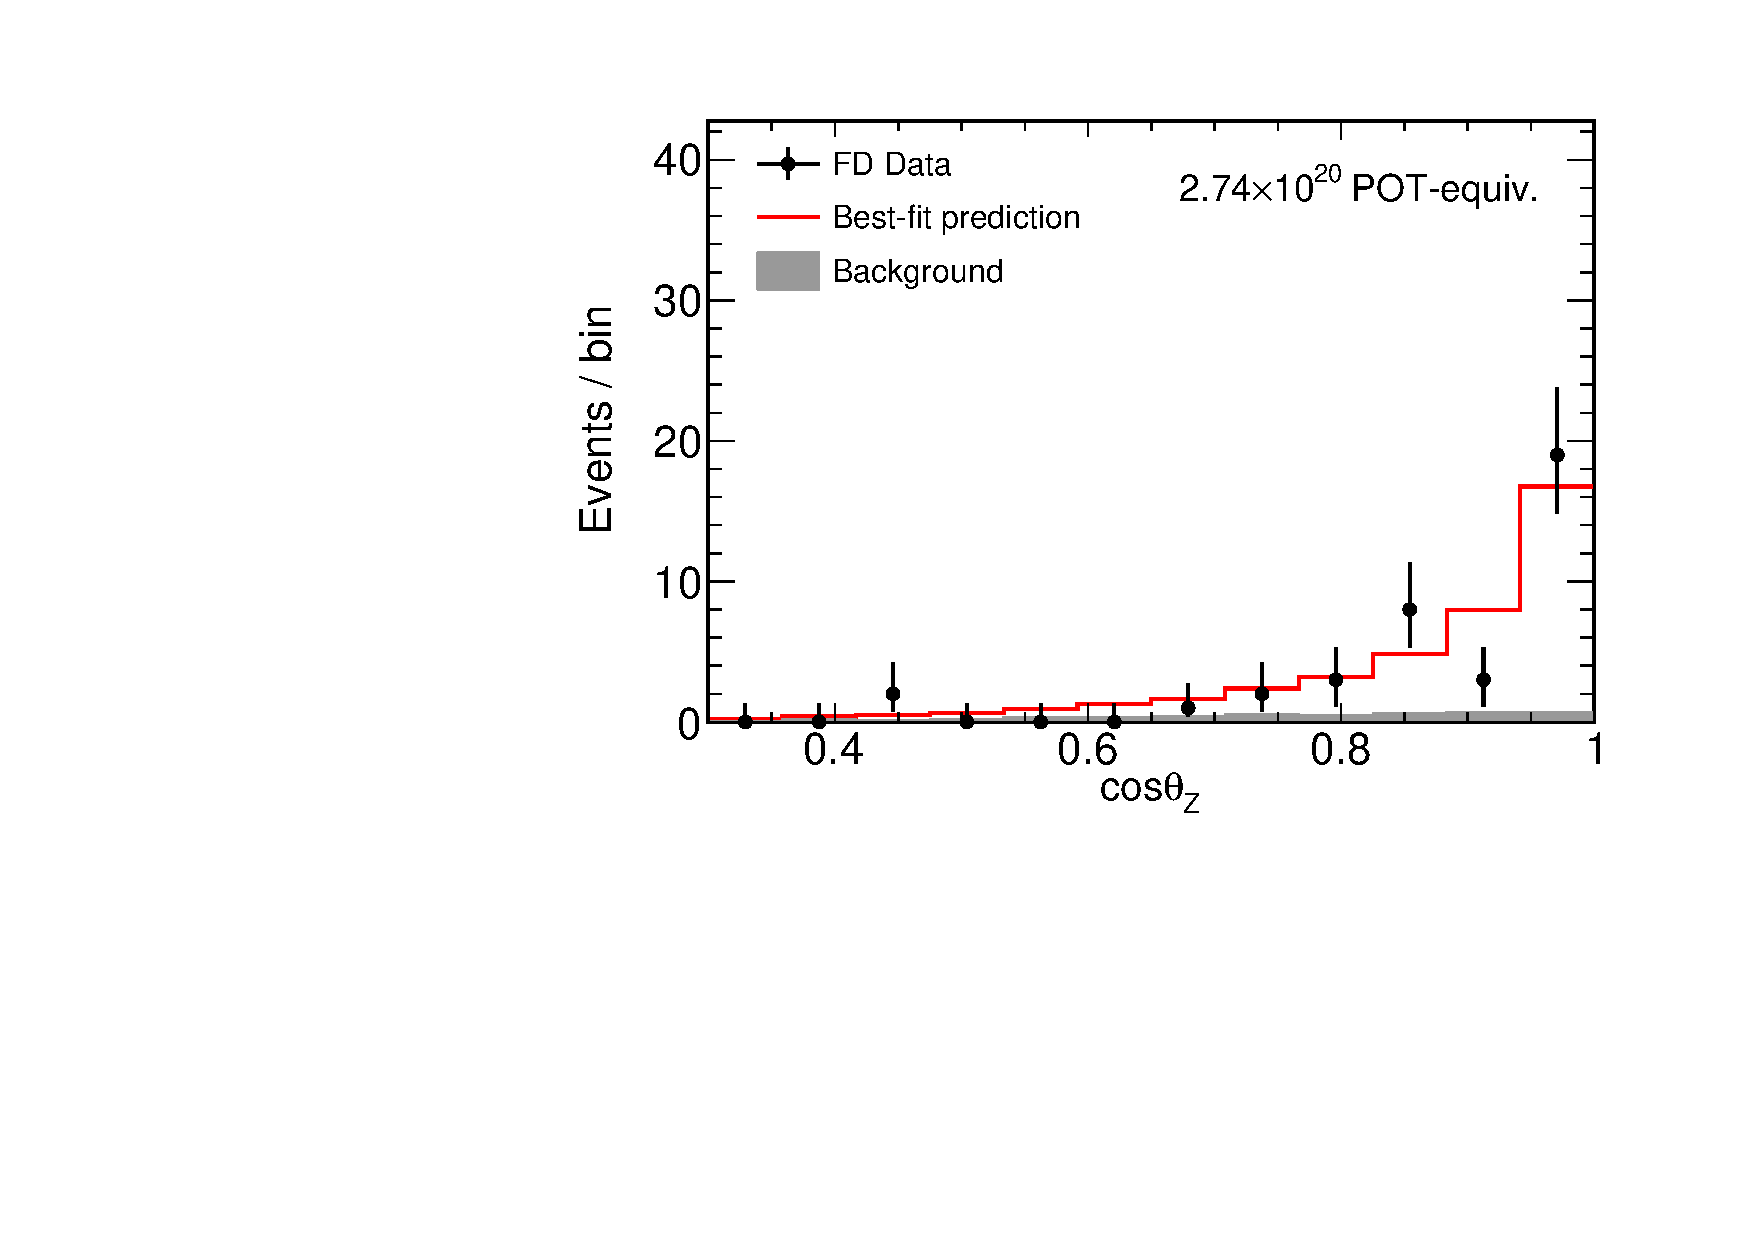
\includegraphics[width=\textwidth]{figures/results/fd_data_mc_numi_plots/dirZ_unblind.pdf}
\end{center}
\caption{  Muon track $Z$-direction cosine distribution for selected FD events with MC prediction }{
The distribution of the 39 selected FD events are shown shown in black.
The selected spectrum was fit to obtain the oscillation parameters used
for the FD MC prediction shown in red, while
the blue dashed line shows the FD MC prediction in the absence neutrino
oscillation.
The background spectrum is shown in gray.
}
\label{dirZ_unblind}

\end{figure}



\begin{figure}
\begin{center}
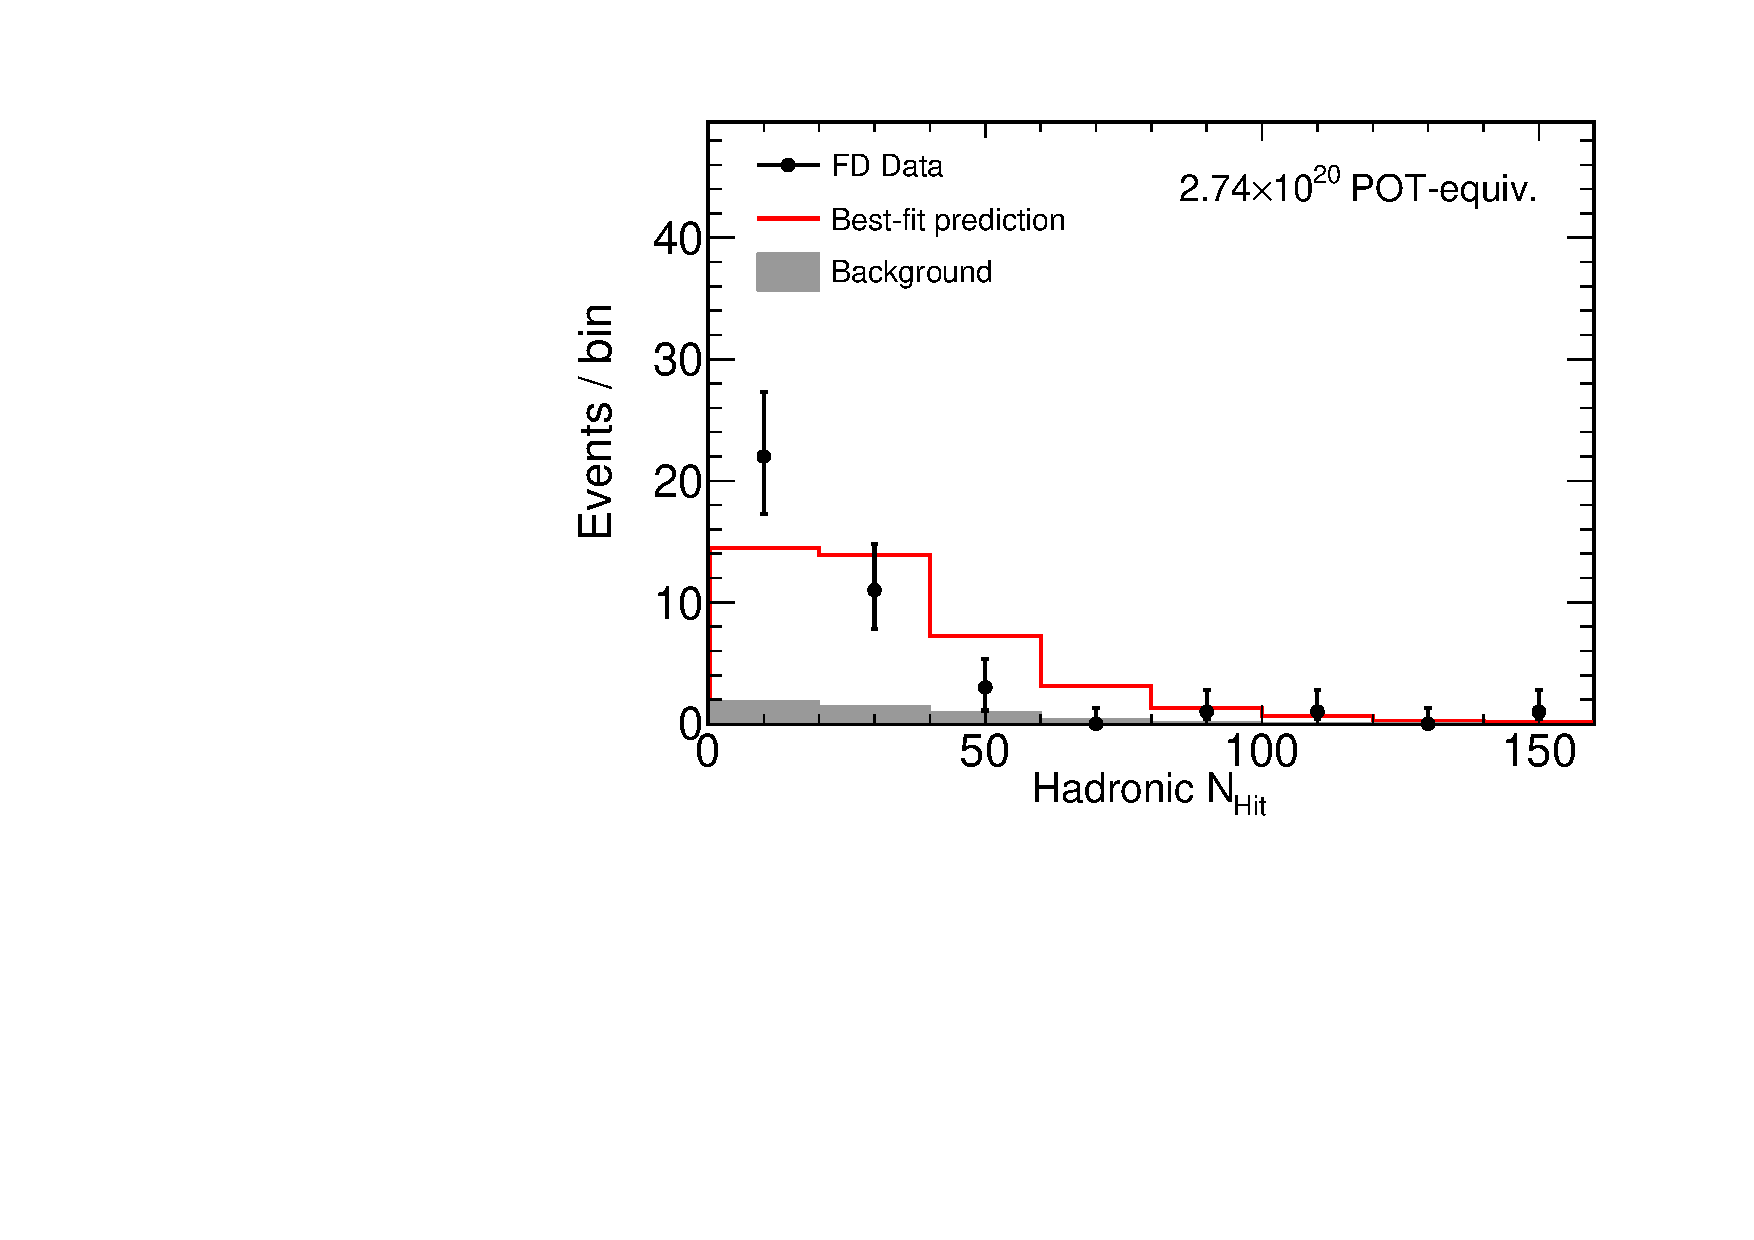
\includegraphics[width=\textwidth]{figures/results/fd_data_mc_numi_plots/hadNhit_unblind.pdf}
\end{center}
\caption{ Hadronic cluster \nhit distribution for selected FD events with MC prediction }{
The distribution of the 39 selected FD events are shown shown in black.
The selected spectrum was fit to obtain the oscillation parameters used
for the FD MC prediction shown in red, while
the blue dashed line shows the FD MC prediction in the absence neutrino
oscillation.
The background spectrum is shown in gray.
}
\label{hadNhit_unblind}

\end{figure}


\begin{figure}
\begin{center}
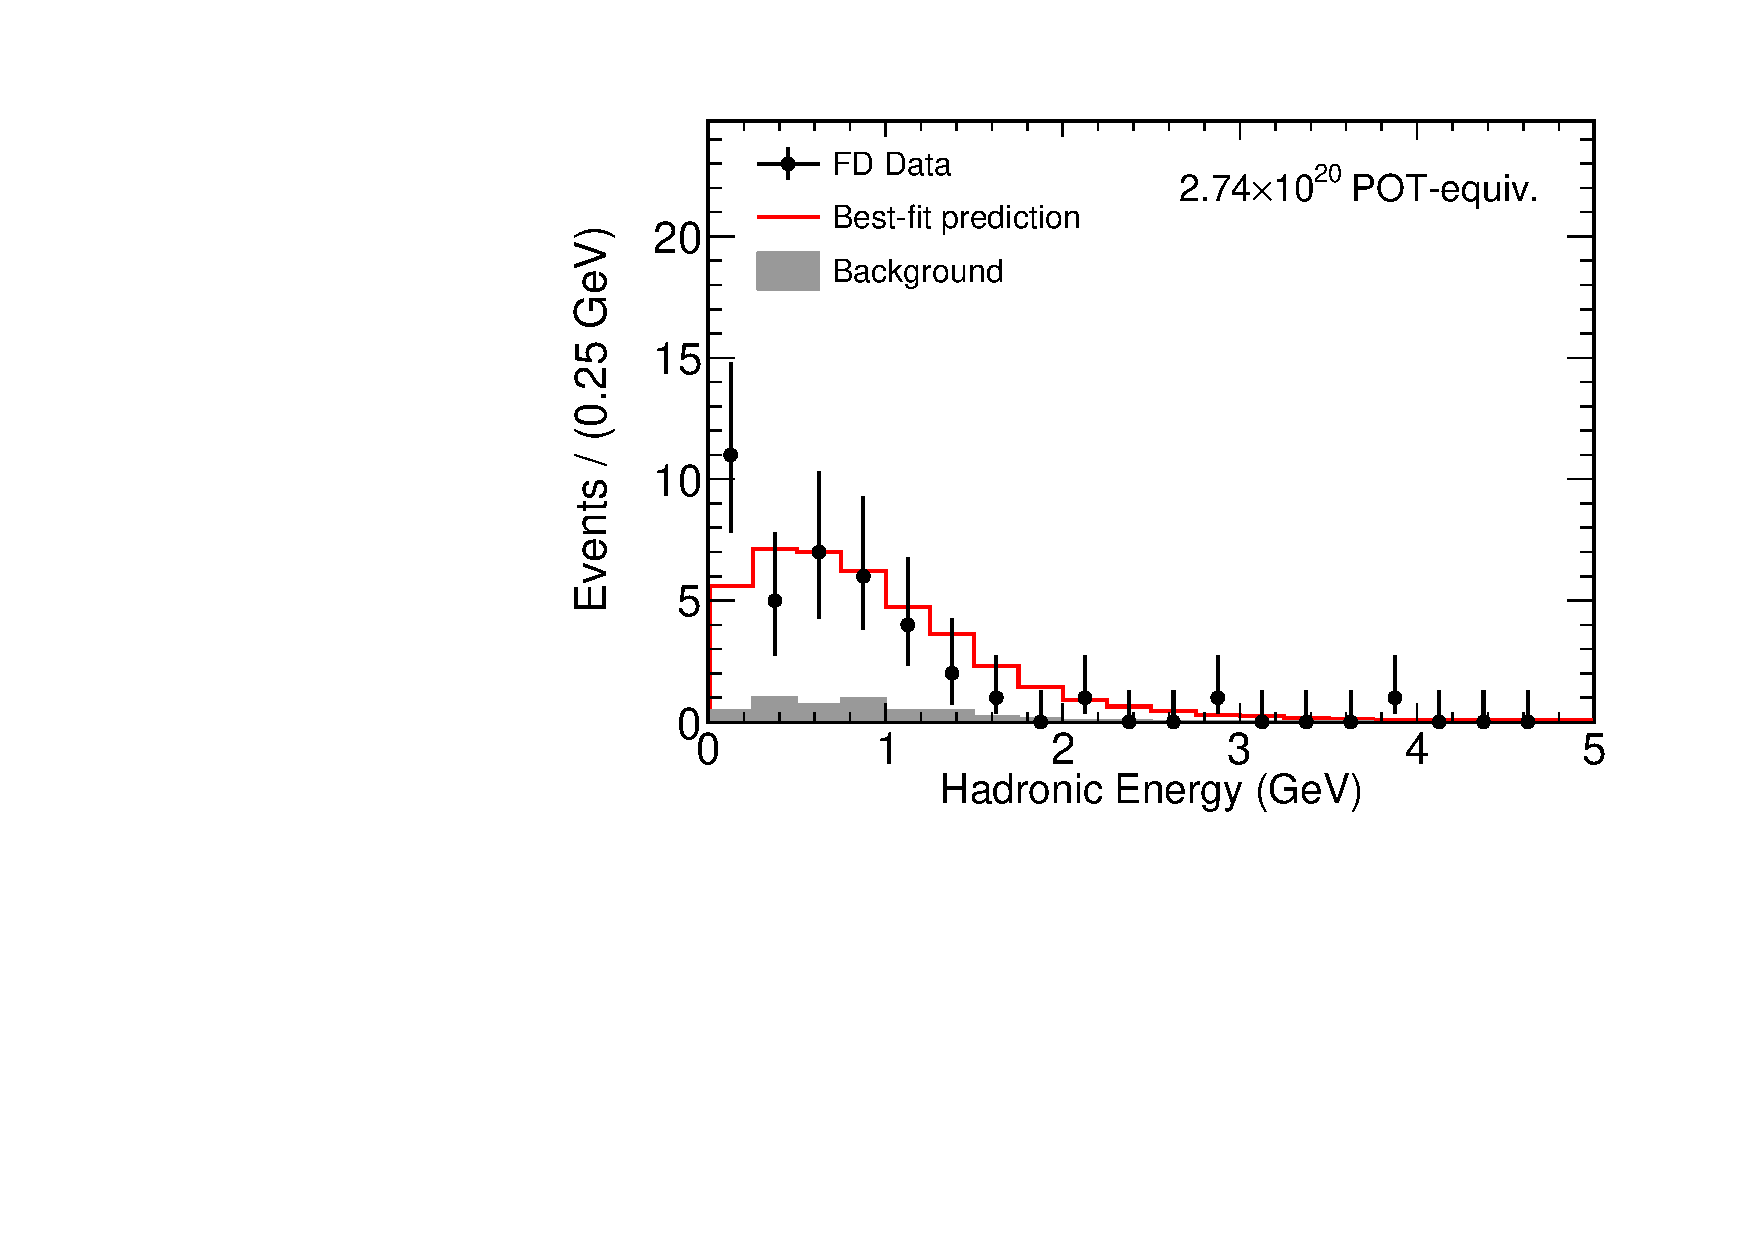
\includegraphics[width=\textwidth]{figures/results/fd_data_mc_numi_plots/hadEshift_unblind.pdf}
\end{center}
\caption{ Hadronic energy distribution for selected FD events with MC prediction }{
The distribution of the 39 selected FD events are shown shown in black.
The selected spectrum was fit to obtain the oscillation parameters used
for the FD MC prediction shown in red, while
the blue dashed line shows the FD MC prediction in the absence neutrino
oscillation.
The background spectrum is shown in gray.
}
\label{hadEshift_unblind}

\end{figure}



\begin{figure}
\begin{center}
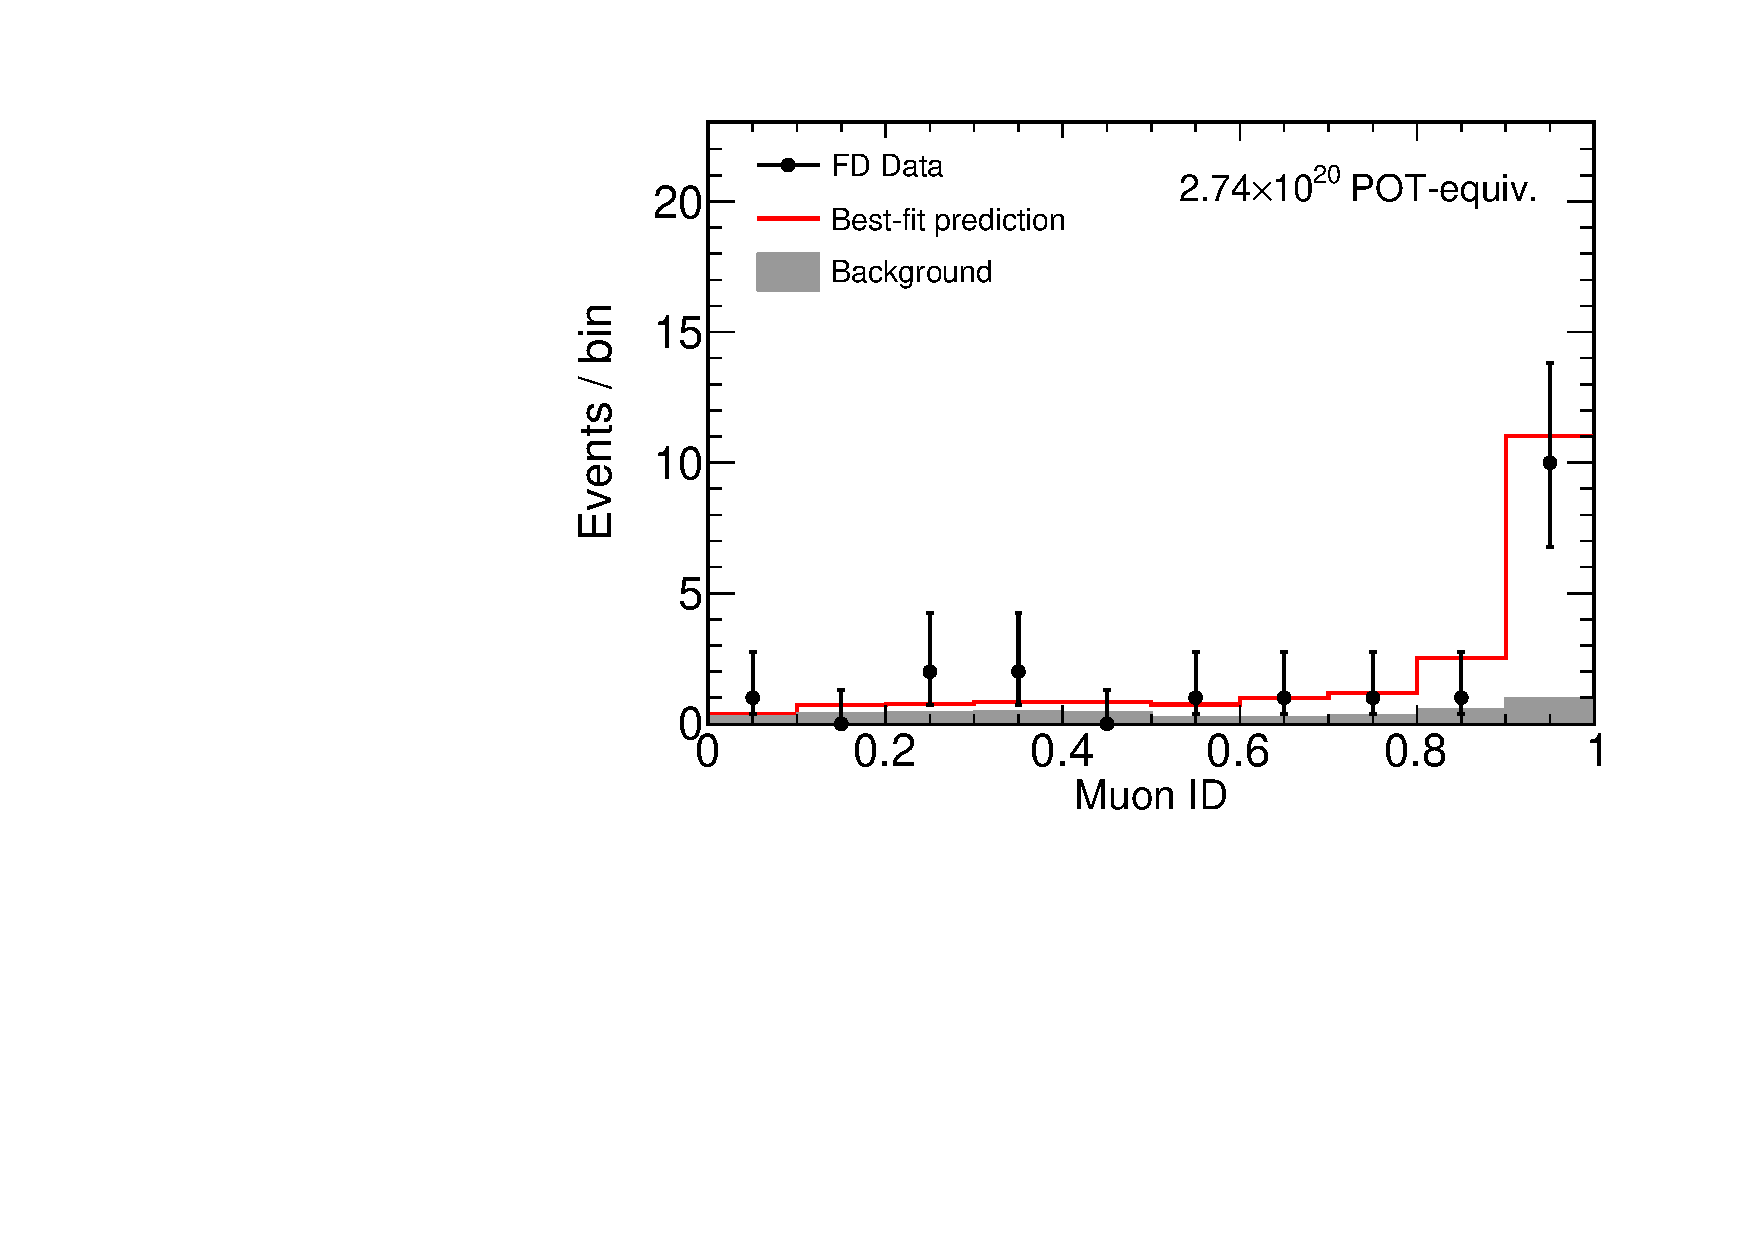
\includegraphics[width=\textwidth]{figures/results/fd_data_mc_numi_plots/remid_unblind.pdf}
\end{center}
\caption{ Muon ID distribution for selected FD events with MC prediction }{
The distribution of the 39 selected FD events are shown shown in black.
The selected spectrum was fit to obtain the oscillation parameters used
for the FD MC prediction shown in red, while
the blue dashed line shows the FD MC prediction in the absence neutrino
oscillation.
The background spectrum is shown in gray.
}
\label{remid_unblind}

\end{figure}


\clearpage

\section{Selected Event Displays}

This section shows a gallery of selected FD events.  Figures \ref{evd_qe_1} and
\ref{evd_qe_2} are candidate \numu CC interactions, Figures \ref{evd_res_1}
and \ref{evd_res_2} are candidate \numu RES interactions,
and Figures \ref{evd_dis_1} and \ref{evd_dis_2} are candidate \numu CC DIS
interactions.





\begin{figure}
\begin{center}
\vspace{-35pt}

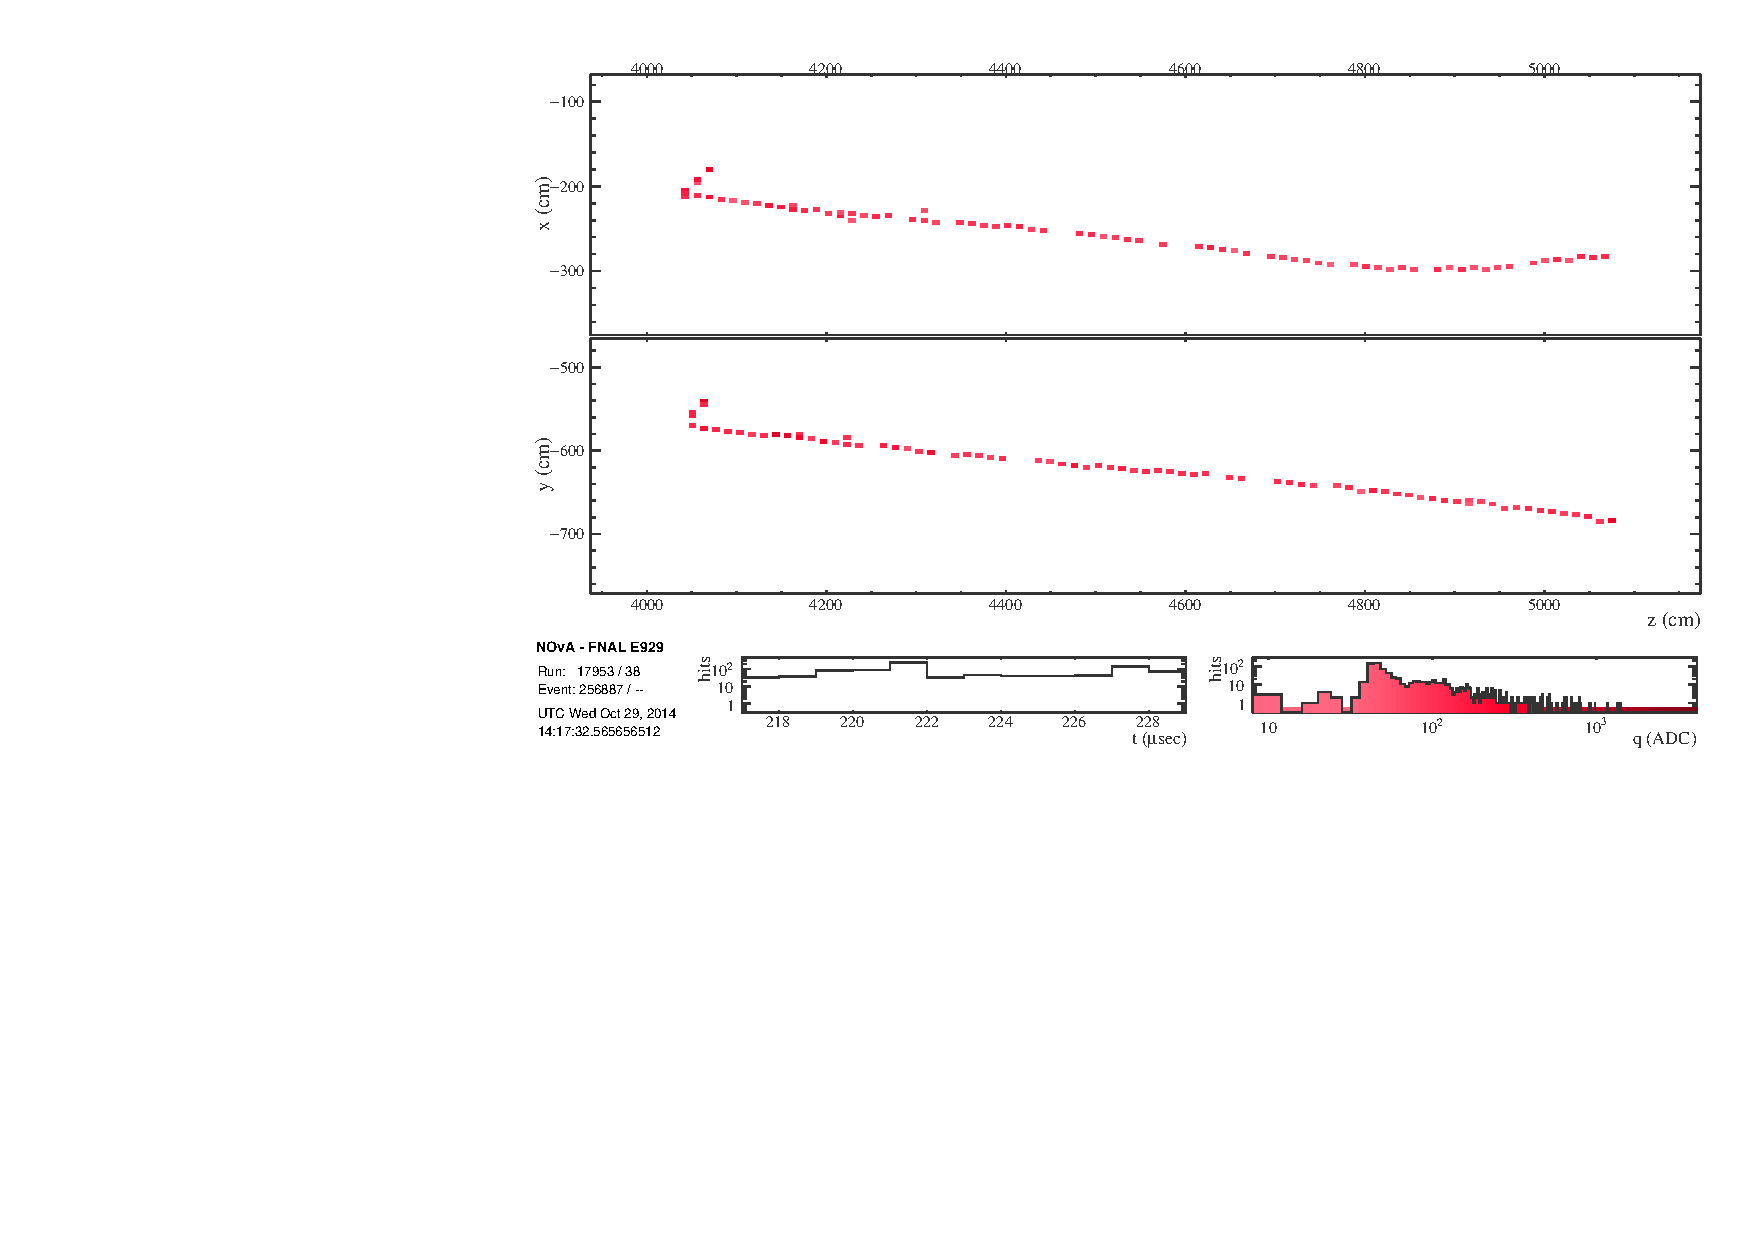
\includegraphics[width=0.87\textheight, angle=90]{figures/results/evd/evd_xzyx-proj_17953_256887.pdf}
\end{center}
\caption{Selected FD \numu CC QE candidate}{
(Rotated left) The top projection is an $X$ vs. $Z$
view, the bottom is $Y$ vs. $Z$.
The bottom left portion of the display
This is a selected \numu charged-current event candidate from the
Far Detector.
With a long muon track and short secondary track, this event bears
the signature of a CC QE interaction.}
\label{evd_qe_1}
\end{figure}
\begin{figure}
\begin{center}
\vspace{-35pt}

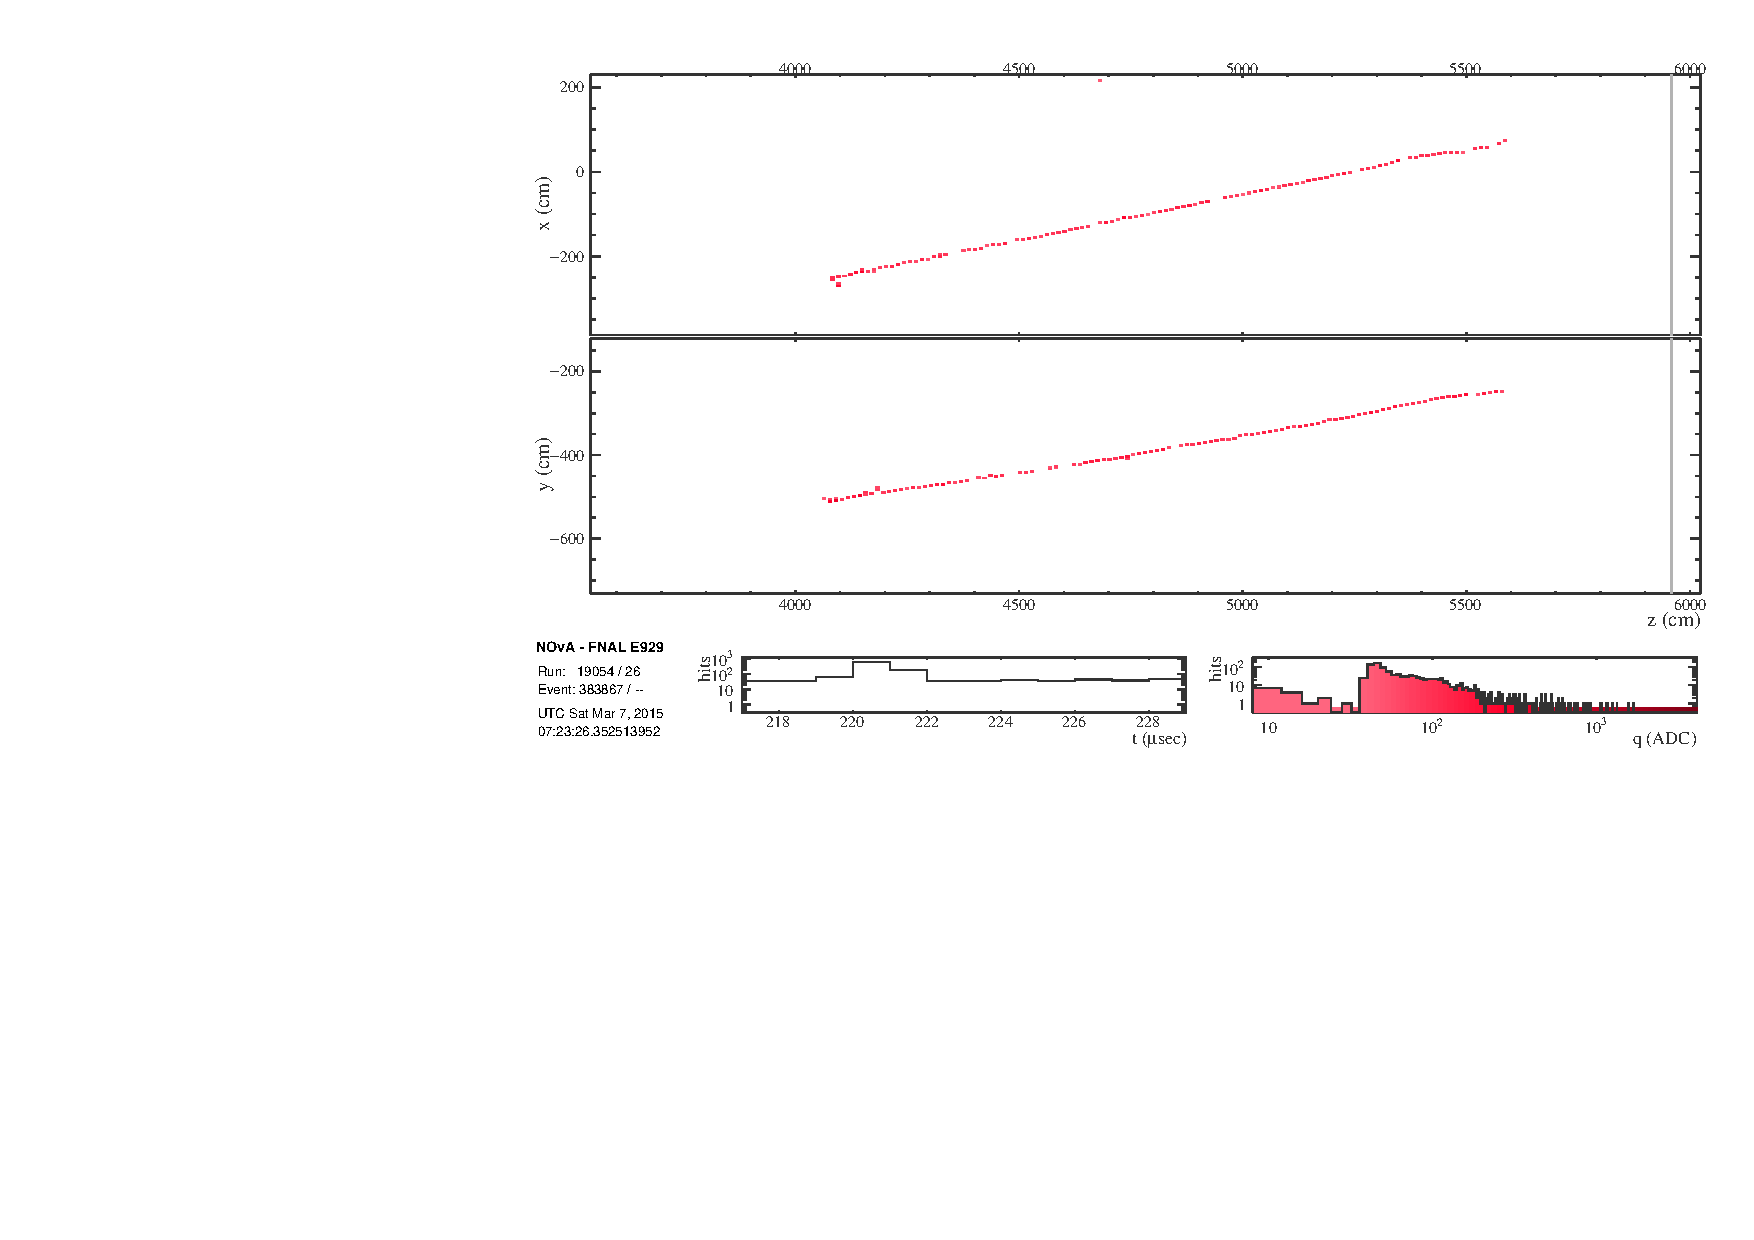
\includegraphics[width=0.87\textheight, angle=90]{figures/results/evd/evd_xzyx-proj_19054_383867.pdf}
\end{center}
\caption{Selected FD \numu CC QE candidate}{
(Rotated left) The top projection is an $X$ vs. $Z$
view, the bottom is $Y$ vs. $Z$.
The bottom left portion of the display
This is a selected \numu charged-current event candidate from the
Far Detector.
With a long muon track and hardly any hadronic activity, this event bears
the signature of a CC QE interaction.}
\label{evd_qe_2}
\end{figure}
\begin{figure}
\begin{center}
\vspace{-35pt}

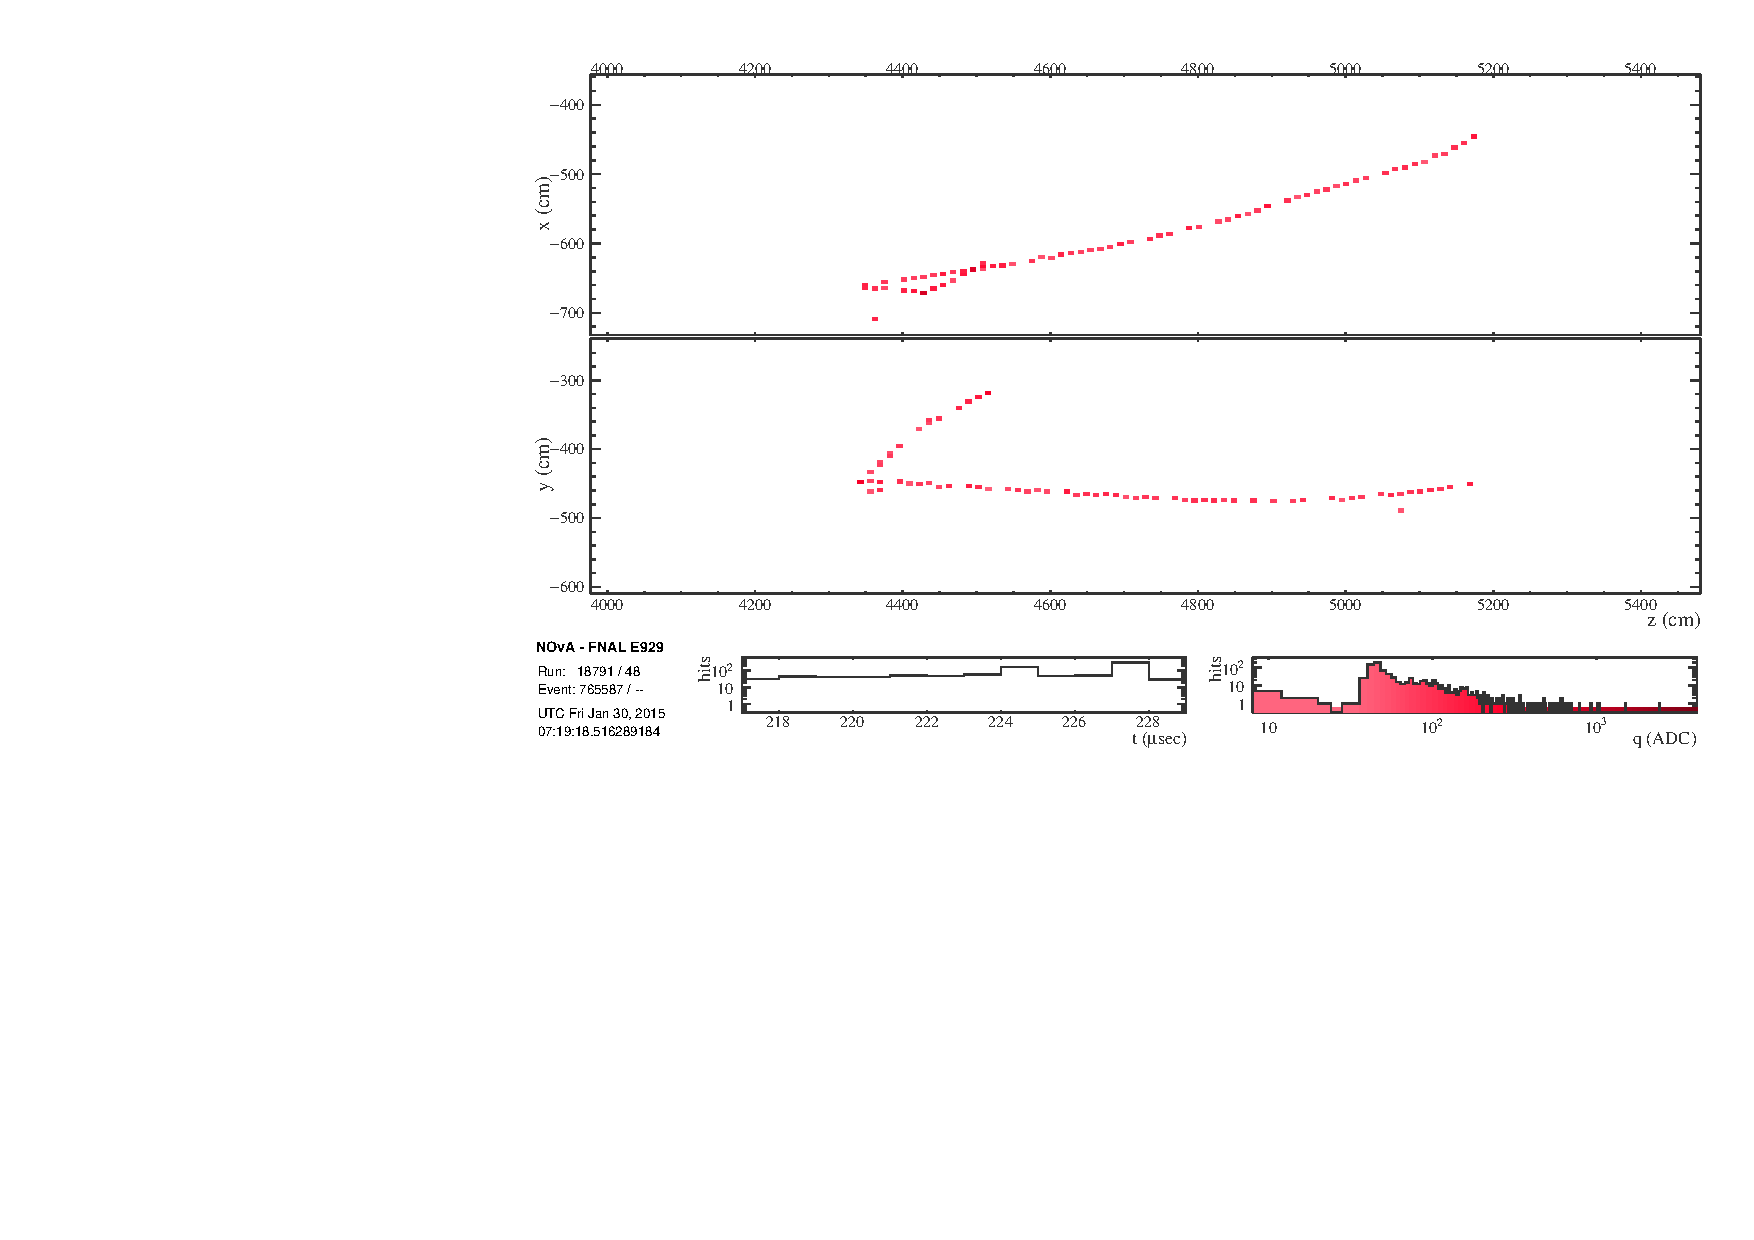
\includegraphics[width=0.87\textheight, angle=90]{figures/results/evd/evd_xzyx-proj_18791_765587.pdf}
\end{center}
\caption{Selected FD \numu CC QE candidate}{
(Rotated left) The top projection is an $X$ vs. $Z$
view, the bottom is $Y$ vs. $Z$.
The bottom left portion of the display
This is a selected \numu charged-current event candidate from the
Far Detector.
The relatively long secondary track possibly a pion, which suggests
this event is a CC RES interaction.}
\label{evd_res_1}
\end{figure}
\begin{figure}
\begin{center}
\vspace{-35pt}

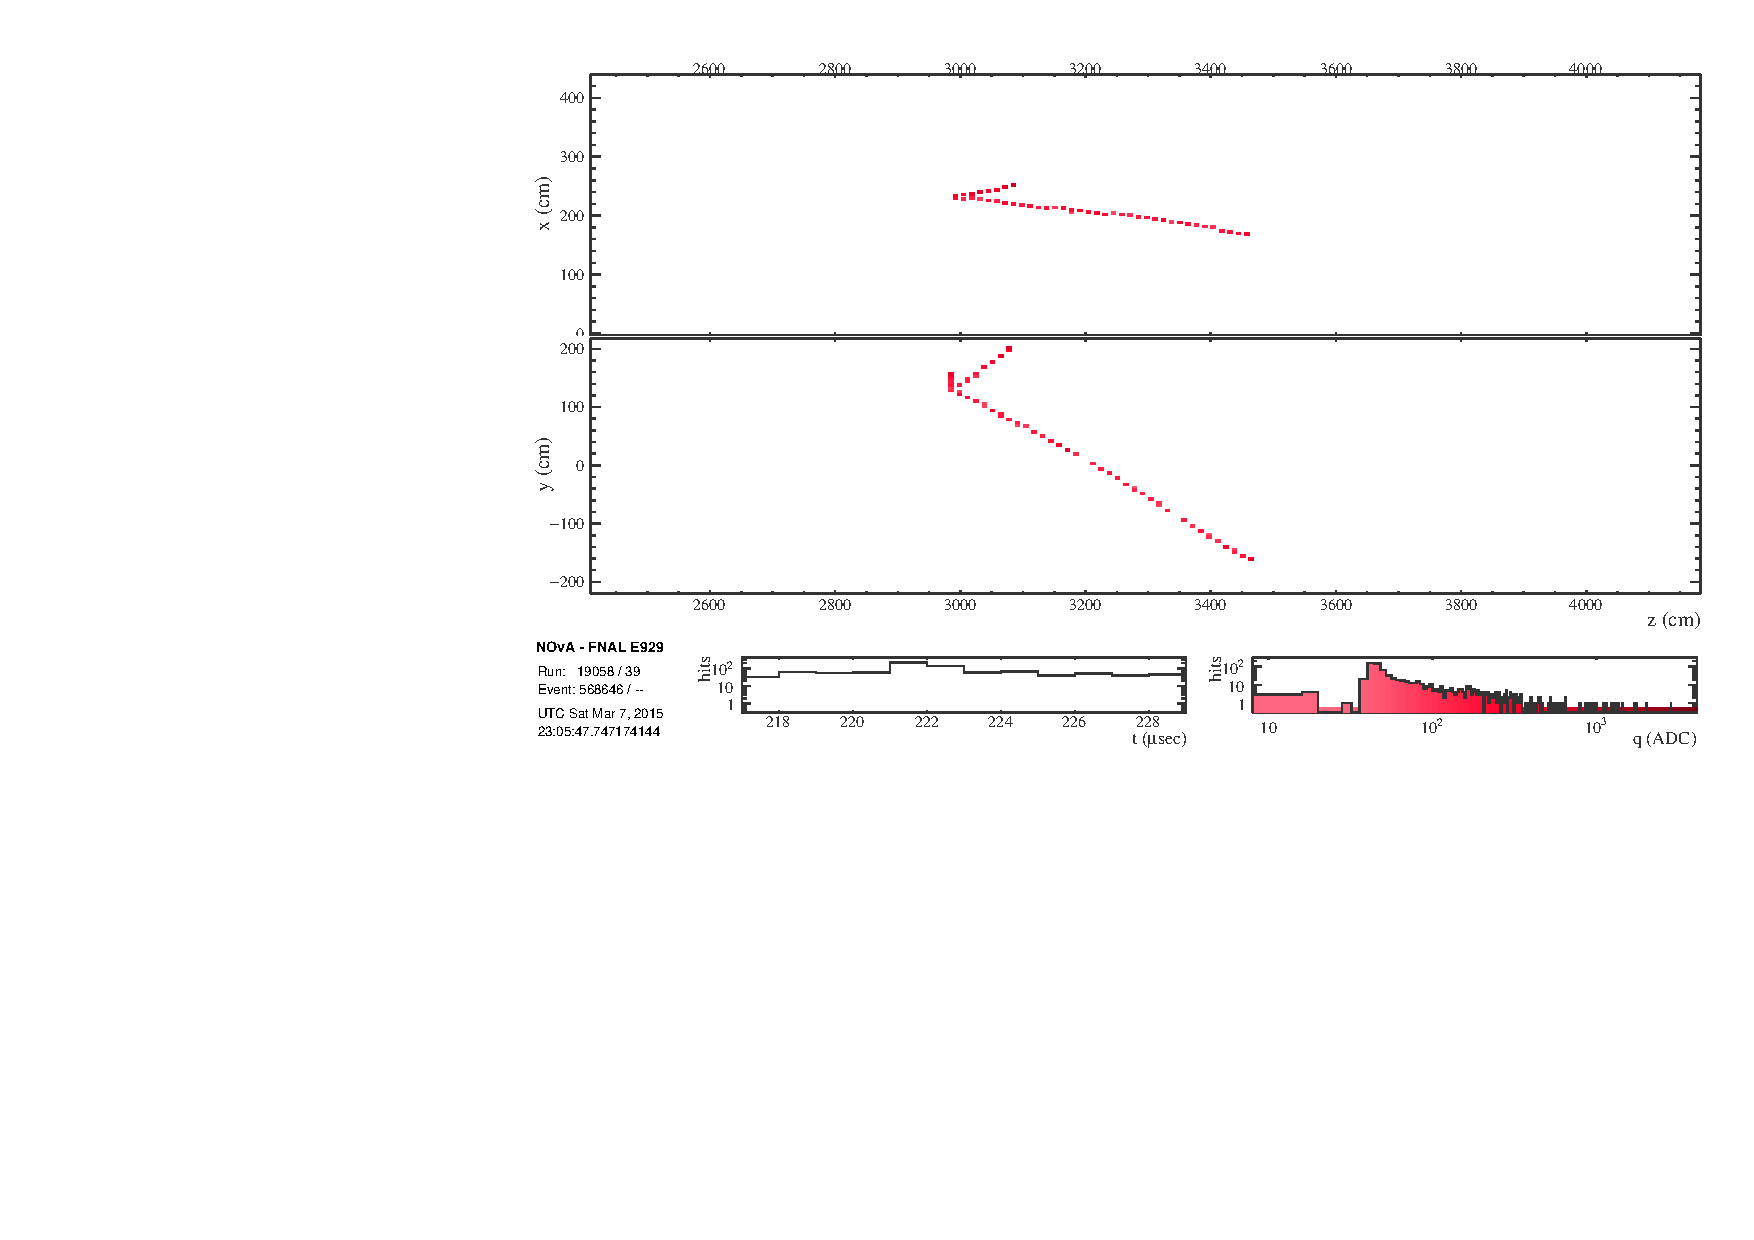
\includegraphics[width=0.87\textheight, angle=90]{figures/results/evd/evd_xzyx-proj_19058_568646.pdf}
\end{center}
\caption{Selected FD \numu CC QE candidate}{
(Rotated left) The top projection is an $X$ vs. $Z$
view, the bottom is $Y$ vs. $Z$.
The bottom left portion of the display
This is a selected \numu charged-current event candidate from the
Far Detector.
The relatively long secondary track possibly a pion, which suggests
this event is a CC RES interaction.}
\label{evd_res_2}
\end{figure}
\begin{figure}
\begin{center}
\vspace{-35pt}

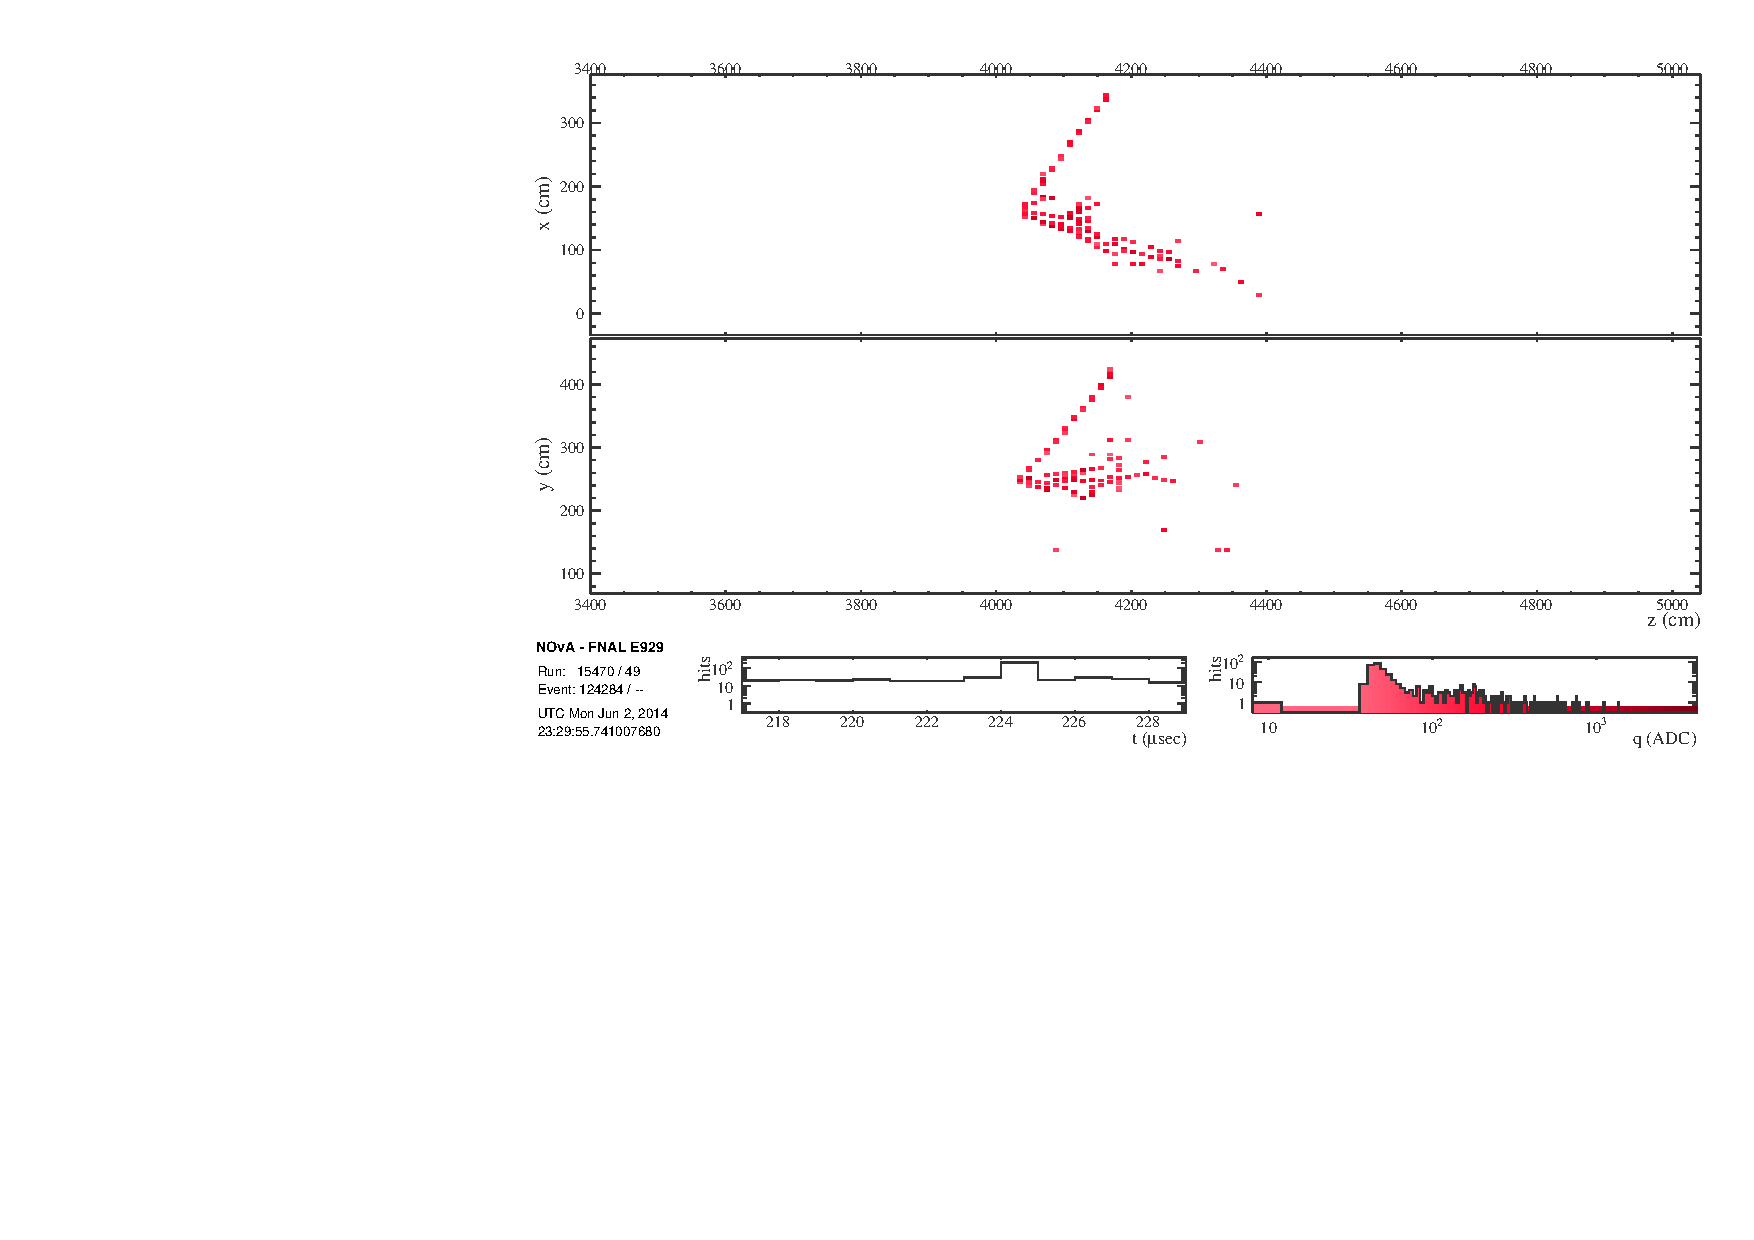
\includegraphics[width=0.87\textheight, angle=90]{figures/results/evd/evd_xzyx-proj_15470_124284.pdf}
\end{center}
\caption{Selected FD \numu CC QE candidate}{
(Rotated left) The top projection is an $X$ vs. $Z$
view, the bottom is $Y$ vs. $Z$.
The bottom left portion of the display
This is a selected \numu charged-current event candidate from the
Far Detector.
The extensive hadronic shower in this event indicates that it could be
a CC DIS interaction.}
\label{evd_dis_1}
\end{figure}

\begin{figure}
\begin{center}
\vspace{-35pt}

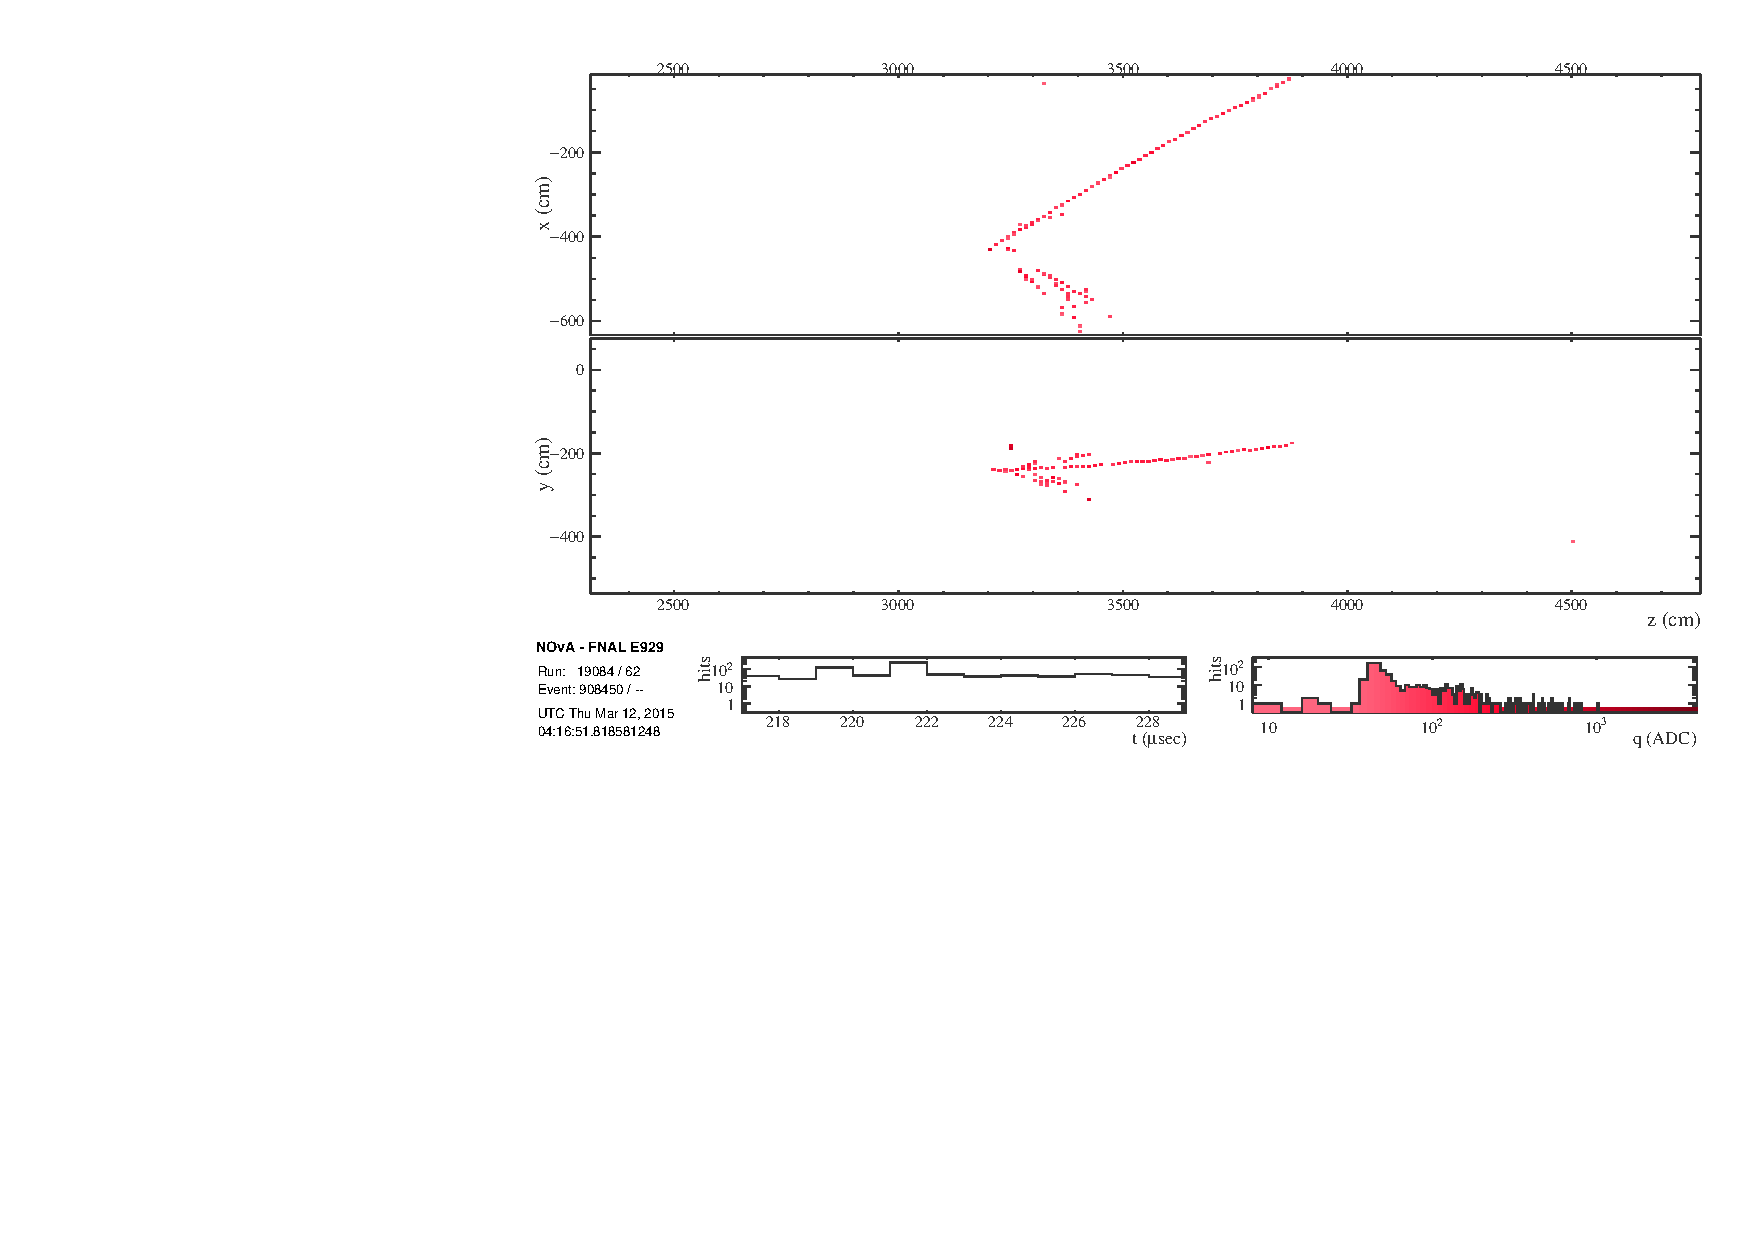
\includegraphics[width=0.87\textheight, angle=90]{figures/results/evd/evd_xzyx-proj_19084_908450.pdf}
\end{center}
\caption{Selected FD \numu CC QE candidate}{
(Rotated left) The top projection is an $X$ vs. $Z$
view, the bottom is $Y$ vs. $Z$.
The bottom left portion of the display
This is a selected \numu charged-current event candidate from the
Far Detector.
The extensive hadronic shower in this event indicates that it could be
a CC DIS interaction.}
\label{evd_dis_2}
\end{figure}

\section{Fit Results}



\label{fit_results_section}
%%%%%%%%%%%%%%%%%%%%%%%%%%%%%%%%%%%%%%%%%%%%%%%%%%%%%%%%%%%%%%%%%%%%%%%%%%%%%%%%
